% #############################################################################
% This is Chapter 2
% !TEX root = ../main.tex
% #############################################################################
% Change the Name of the Chapter i the following line
\fancychapter{Background}
\cleardoublepage
% The following line allows to ref this chapter
\label{chap:back}

	The development of an algorithmic-based framework for optimization, applicable to architectural domains, requires a careful review over the current literature on \ac{BPO} practices and their limitations. 
	
	Firstly, building design is a multi-disciplinary practice that involves a wide variety of different problems. According to their characteristics, some optimization algorithms may be more or less adequate to address them, as algorithms often adopt different strategies or techniques. To maximize the potential of the optimization, it is therefore necessary to distinguish between different problems and which optimization algorithms are more suitable for which problems. One important distinction is between single- and multi-objective problems. Generally, \ac{BPO} practices require the optimization of multiple aspects simultaneously, a multi-objective problem. However, this objectives' multiplicity instills performance issues that must be properly addressed. This chapter discusses four different approaches to address these problems.
	
	Secondly, the costly nature of the functions used for performance assessment in \ac{BPO} motivates the application of a special class of optimization algorithms, the derivative-free algorithms. Within this class, different categories emerge, emphasizing the algorithms' different properties and search strategies. Applying the adequate algorithm to certain problems may potentially increase the efficiency of optimization processes, especially for problems involving time-consuming evaluations.
	
	Finally, the development of design optimization tools fostered the coupling between optimization and design practices. Currently available architectural optimization tools optimize the parametric models produced in the visual programming environments, like Grasshopper and Dynamo. These environments are closely integrated within \ac{CAD} and \ac{BIM} tools, respectively, hence enabling a seamless and friendlier association between optimization tools and typical \ac{BPO} design workflows. Also, the \textit{ready-to-use} format of these optimization tools' interfaces are very appealing to most \ac{BPO} practitioners~\cite{Cichocka2017SURVEY}.
	
	After a comprehensive description of the previously mentioned views of \ac{BPO} practices, in \Cref{sec:problemsaddress}, we emphasize the main limitations of currently existing \ac{BPO} practices. 
	
\section{Optimization Problems}
\label{sec:optimizationproblems}
	
	Generally, an optimization process consists in two main parts: modeling and optimization algorithms. Covered in this section, the first part involves the creation of a model representing the system or problem to optimize, while the second part, further discussed in \Cref{sec:optimizationalgorithms}, focus on the application of a strategy capable of searching among the set of possible solutions, i.e., the solution space, for optimal solutions.
	
	An optimization process often starts with the formulation of the model of the system or problem to address, in a process known as modeling. The model is described in terms of (a) the variables or unknowns, which represent the system's or problem's characteristics, (b) the objectives or criteria, representing the quantitative measures of the system's performance, which are usually functions of the variables, and, optionally, (c) the constraints, representing the conditions that have to be satisfied to guarantee the system's feasibility~\cite{Nocedal2011NumericalOptimization}. 
		
	There are numerous possibilities to create optimization models, each yielding a different mathematical classification. Concretely, models variability include, among others, the variable types, the presence or absence of constraints, and the number and nature of the objective functions. In addition to the model, the search strategies can also be classified according to the scope of the search, i.e., whether they explore vaster or narrower regions of the solution space. 
	
	Particularly, in \ac{BPO}, building designs may yield different optimization problems, depending on the way they are modeled and the limitations or restrictions imposed by architects or engineers. For example, in order to reduce fabrication costs it is very frequent to limit the granularity of the design's components to vary within certain values. As another example, consider the situation where, to preserve the architect's intention, building designs are confined to have specific shapes (e.g., arc-shaped, round-shaped, squared-shaped) and each shape can be varied according to some defined parameters. Moreover, it is also possible that when building design becomes more complex, architects decide to relax some of the previously established conditions. Indeed, as it will be further discussed in \Cref{ssec:soo,ssec:preferencesarticulation}, when facing problems involving the simultaneous expensive evaluation of multiple performance aspects, time restrictions often force architects to abdicate some performance aspects, or, in some cases, to define a preference amongst the considered performance aspects.
	
	
\subsection{Problems Classification}
	
	The mathematical optimization field offers different classifications for optimization problems. In this chapter, we introduce three of these classifications due to their relevance and their ubiquitousness for optimization problems. \Cref{fig:optclassification} exhibits a schematic representation of the four different optimization classifications considered in this dissertation (the fourth classification will be discussed in \Cref{sec:optimizationalgorithms}). For a more comprehensive treatment of this subject, consider~\cite{Nemhauser1988,Nocedal2011NumericalOptimization}. 
	 
	The first classification differentiates \textbf{continuous} and \textbf{discrete} optimization problems depending on the variables' types. Continuous optimization refers to problems defined uniquely by continuous variables and, therefore, characterized by an infinite solution space, whereas discrete optimization refers to problems for which some or all their variables are discrete, hence yielding a finite solution space. In continuous optimization, the smoothness of functions make it possible to reason about the behavior of all points close to $x$ and, consequently, to solve these problems more easily, whilst the commonly present irregularities of discrete optimization functions do not, in general, allow to draw any information about the behavior of points close to $x$. Discrete classification encloses finer optimization classes, such as integer optimization or combinatorial optimization~\cite{Nemhauser1988}. 
	
	The second classification relates to the presence of constraints on the variables. \textbf{Unconstrained} optimization problems result from many practical applications and have no restrictions on the variables' values. Contrastingly, \textbf{constrained} optimization problems usually emerge from systems where constraints are crucial (e.g., economy problems, imposing cargo constraints) and are incorporated them into the problem's definition. Variables can be restricted using hard or soft constraints. Hard constraints set conditions for the variables that must be satisfied, namely, to vary within simple bounds (e.g.: $-1<x<1$) and to relate to other variables in certain ways (e.g.: $\sum_{i} x_i$), whereas soft constraints set penalties for the variables whose value violates the condition. Constrained optimization problems are often converted to unconstrained ones by replacing hard constraints with soft constraints, i.e., by adding penalization terms in the objective function to discourage the violation of constraints~\cite{Nocedal2011NumericalOptimization}. 

	The third, and final, dichotomy herein discussed focuses on the number of objectives to optimize, which can be distinguished in \textbf{single-objective} and \textbf{multi-objective}. \ac{SOO} focus on the optimization of one objective, whilst \ac{MOO} focus on problems involving multiple conflicting objectives simultaneously. Besides the larger objectives' number, addressing multi-objective problems also entails more complex optimization problems. For problems involving time-consuming evaluations, the increased complexity jeopardizes the executability of optimization and spurs the adoption of other, often simpler, approaches. The following sections describe different approaches to single- and multi-objective optimization problems. 
	
	\todo{Put picture with the scheme - make in ppt}
	\begin{figure}
		\centering
		
\includegraphics[width=5cm]{Images/placeholder-image.png}
		\caption{Different classifications of optimization processes.}
		\label{fig:optclassification}
	\end{figure}
	
	% ----------- 
	\subsection{Design of Experiments}
	\label{ssec:doe}
	
	The experimental or design of experiments approach is widely used in research and in practice to address both single and multi-objective problems~\cite{Fang2017}. Besides being intuitive and flexible, it can achieve a potentially better solution without having to deal with complex optimization algorithms. This approach evaluates designs generated with different combinations of design parameters. These combinations can be obtained through sampling methods, such as Full-factorial, Monte Carlo Sampling, or Latin Hypercube Sampling~\cite{Giunta2003DOE}, which generate different variations of the design to be evaluated. This approach returns multiple design solutions instead of just one, leaving the final choice in the hands of the architect.
	
	Unfortunately, this approach does not guarantee that good solutions will be found. In fact, in most cases, new solutions are generated without taking advantage of the information obtained from previously evaluated designs. Consequently, the old information is not used to guide the search towards the most efficient designs and useless candidate designs can sometimes be evaluated. 
	
	On the other hand, given its simplicity and flexibility, this approach allows architects to easily combine different processes in order to direct the search towards better design solutions. For example, the architect can choose a sampling method to generate different design variations, which are then evaluated. After analyzing the results of the evaluations, the architect may wish to explore regions of the design space near the most promising design solutions. In that case, he might constrain the design variations to lie within the promising regions, by updating the problem’s definition. The redefined problem is then subsequently sampled and redefined until the architect is satisfied with the quality of the obtained solutions.
	
	Despite the constant need for manual intervention, the previous technique can be adapted to automatically extract information about the design problem itself, for example, to study the impact of design parameters in the performance. This process, commonly known as \textit{sensitivity analysis}~\cite{Saltelli2007}, has already been applied in the context of building design optimization~\cite{Tian2013}, not only to achieve better solutions, but also to enhance the performance of existing optimization algorithms, e.g., by dropping irrelevant parameters.
	
	Overall, while it does not provide guarantees about the solutions’ optimality, this approach is simple, easy to use, and it is available in numerous tools. Moreover, although this process is not intelligent \textit{per si}, since the decisions are always made by the architect, it enables a more informed design process, as it presents all the design variations generated and their associated performance.
	
	% #############################################################################
	\subsection{Single-Objective Optimization}
	\label{ssec:soo}
	
	\ac{SOO} processes aim to find the best solution with respect to a unique objective function. This function is described in terms of the values of the problem's parameters. \Cref{eq:soo} illustrates an example of a mathematical constrained minimization \ac{SOO} problem, where $f$ represents the single-objective function, $g_j$ and $h_k$ represent the constraints to be satisfied, and $x$ represents the parameters' vector.
	
	\begin{equation} \label{eq:soo}
	\begin{aligned}
	& \underset{x \in \mathbb{R}^n}{\text{minimize}}
	& & f(x) \\
	& \text{subject to}
	& & g_j(x) = 0, & \; j &= 1, \ldots, J, \\ 
	&&& h_k(x) < 0, & \; k &= 1, \ldots, K.
	\end{aligned}
	\end{equation}
	
	Generally, the computational complexity of optimization processes is exponential on the number of objectives and, consequently, the more objectives, the more expensive processes are. In particular, \ac{SOO} processes rely exclusively on a single objective function and are, therefore, usually less time-consuming than \ac{MOO} processes. The main difference between these two processes is that the former focus on finding the solution that optimizes a single function, whereas the latter focus on finding the optimal trade-offs between the, potentially conflicting, multiple objective functions. The difference in the computational resources become particularly relevant when considering simulation-based objective functions, as these tend to be very time-consuming. 
	
	Particularly, in the case of building design, because most problems include simulation-based objective functions, architects commonly opt for \ac{SOO} processes~\cite{Wortmann2017Opossum}: either by simply considering a single performance aspect (or objective), or, in the case of problems involving multiple conflicting aspects, by combining them in a unique function as it will be further explained in \cref{ssec:preferencesarticulation}.
	
	A literature review over the architectural practice will evidence the prevalence of \ac{SOO} practices. Firstly, single-objective problems are easier to model. Secondly, available optimization plug-ins, like Galapagos and Goat, allow to easily address single-objective building design problems. As a result, not only are architects capable of solving these optimization problems, but, when facing more complex \ac{MOO} problems, they are also encouraged to adopt simplified versions of such problems, thus reducing the overall complexity of those optimization processes. Finally, the variety of optimization algorithms exposed in these plug-ins enables the selection of the best algorithm to specific problems, thus spurring more efficient optimization processes~\cite{Wortmann2016BBO}.  
	
	Although \ac{SOO} yields less time-consuming processes, these are also less informative than \ac{MOO}, as they usually focus on a single optimal solution. As a case in point, building design often involve different conflicting aspects (e.g., thermal, energy consumption, cost), for which information about the different compromises would aid in the comprehension and making of more informed decisions.
	
	% #############################################################################
	\subsection{\textit{A Priori} Articulation of Preferences}
	\label{ssec:preferencesarticulation}
	
	This approach comprises a simplified way of handling \ac{MOO} that is very resemblant of the \ac{SOO} approach previously discussed, but without disregarding any of the performance aspects. Particularly, this approach combines multiple objective functions according to one’s preferences, using what is called a utility function \cite{Marler2004}, i.e., a function which ranks alternatives according to their utility for global performance. 
	
	Among all the possible utility functions, the most common one is the weighted sum~\cite{Wortmann2017Opossum}, also referred to as linear \textit{scalarization}, in the literature. This utility function reduces \ac{MOO} to \ac{SOO} problems by weighting the different objectives and combining them into a single function, as depicted in~\Cref{eq:scalarization}. The weights ($w_i$) assigned to each objective function ($f_i$) represent their relative importance to the architect and they must be set during the modeling of the optimization problem, that is, before starting the search for optimal solutions. The resulting function is then provided to a \ac{SOO} algorithm as the function to optimize. 
	
	\begin{equation} \label{eq:scalarization}
	\begin{aligned}
	& \underset{x \in \mathbb{R}^n}{\text{minimize}}
	& & \sum_{i=1}^n w_i f_i(x), & \; i &= 1, \ldots, n, \\
	& \text{subject to}
	& & g_j(x) = 0, & \; j &= 1, \ldots, J, \\ 
	&&& h_k(x) < 0, & \; k &= 1, \ldots, K.
	\end{aligned}
	\end{equation}
	
	Despite its similarity to \ac{SOO}, this approach incurs into a much more computationally complex process than the latter one, as it still involves the evaluation of multiple objective functions. As a result, the time complexity process is considerably increased and, instead of taking seconds, minutes, hours, or days, per function evaluation, takes that value multiplied by the number of objectives. Nevertheless, this approach still manages to be less time-consuming than the analogous Pareto-based \ac{MOO} approach (that will be discussed in \Cref{ssec:pareto}), as it focus on the optimization of a single preference, instead of attempting to find the trade-offs among all the objectives. 
	
	As a case in point, in architecture, this approach is particularly useful, when more experienced architects can use additional knowledge to define an appropriate set of preferences, instead of resorting to the analogous Pareto-based approach, which would yield a far more complex optimization process. In terms of the impacts in the design process itself, this approach yields a more intelligent, but less informed design process. On the one hand, it confers intelligence because the involved optimization algorithms usually exploit the knowledge of previously evaluated solutions to guide the search towards optimal regions of the design space. On the other hand, it is less informed, because architects no longer control or have information about the optimization process. The loss of control results from the automated character of the optimization algorithms involved in the architectural practice, which frequently exclude architects from the optimization loop. As a consequence, in general, the architect has no information about the solutions evaluated during the optimization process and is only provided with a single solution\footnote{The interest in having a subset of optimal solutions led to the development of mechanisms to provide a subset of optimal solutions instead of a single one.}. The lack of information is perceived as a limitation ~\cite{Cichocka2017SURVEY} and it restricts the architect to either comply with the retrieved solution or to rerun the optimization again. Either way, this optimization approach does not provide in general enough information to understand the optimization results, and, consequently, make more informed decisions. 
	
	Overall, in architectural domains, the virtues of this approach include the ease of use, the availability, the heterogeneity of ready-to-use \ac{SOO} tools (e.g., Opossum, Goat, Galapagos, Silvereye), and the time complexity. %when compared to other \ac{MOO} approaches. % In general, because this preference-based approach focus in the retrieval of a single optimal solution that satisfies the previously defined preferences, it becomes more effective and less time consuming than other \ac{MOO} approaches, that either lack a more guided search or that aim at finding solutions that are optimal under different preference articulations. 
	
	% #############################################################################
	\subsection{Pareto-based Optimization}
	\label{ssec:pareto}
	
	Despite allowing to handle \ac{MOO} problems, the previous approach does not consider the different trade-offs among the potentially conflicting objectives, instead forcing the user to make an \textit{a priori} decision regarding the importance of each objective. Pareto-based optimization approaches attempt to address this limitation by postponing that decision until the end of the optimization process. In this approach, all objectives are taken as equally important during the optimization, making it more difficult to discern the quality of each solution. In other words, while in \ac{SOO} problems, we expect the optimal solution to be the set of parameters' values that achieve the best\footnote{For simplification purposes, we simply refer to the optimal solution as being the best. When dealing with a minimization problem, the best solution is the one that achieves the lowest value of the objective function, whereas in maximization problems, the best solution is the one achieving the highest value of the objective function.} objective value possible, in \ac{MOO}, the best possible configuration for one of the objectives is rarely the best possible configuration for all other objectives, which results from the fact that these objectives are often contradictory. \Cref{eq:pareto-based} presents an example of the mathematical definition of a constrained minimization \ac{MOO} problem, where $F(x)$ represents the vector of $k$ objectives, $f_i$ represent the $i^{th}$ objective function, $g_j$ and $h_k$ represent the constraints to be satisfied, and $x$ represents the parameters' vector.
	
	\begin{equation} \label{eq:pareto-based}
	\begin{aligned}
	& \underset{x \in \mathbb{R}^n}{\text{minimize}}
	& & \left\lbrace F(x) = \left[f_1(x), f_2(x), ..., f_n(x)\right]  \right\rbrace \\
	& \text{subject to}
	& & g_j(x) = 0, & \; j &= 1, \ldots, J, \\ 
	&&& h_k(x) < 0, & \; k &= 1, \ldots, K.
	\end{aligned}
	\end{equation}
	
	In order to assess the quality of multi-objective solutions, it becomes necessary to apply a new optimality criterium, like the Pareto optimal (or Pareto efficient) concept. Named after the economist Vilfredo Pareto, the Pareto optimal concept defines an optimal solution as being a solution for which it is impossible to improve an objective value without deteriorating others. Such a solution is also said to be non-dominated or noninferior, and the set of non-dominated solutions is called the Pareto front. An example of a bi-objective minimization problem is illustrated in \Cref{fig:paretofrontier}. The two objectives are $f_1$ and $f_2$, and the solutions shown in orange are non-dominated. The goal of Pareto-based optimization algorithms is to find design solutions that lie on the Pareto front.
	
	% Begin Pareto-Optimization Figure -------------------------------------------------------
	\begin{figure}
		\centering
		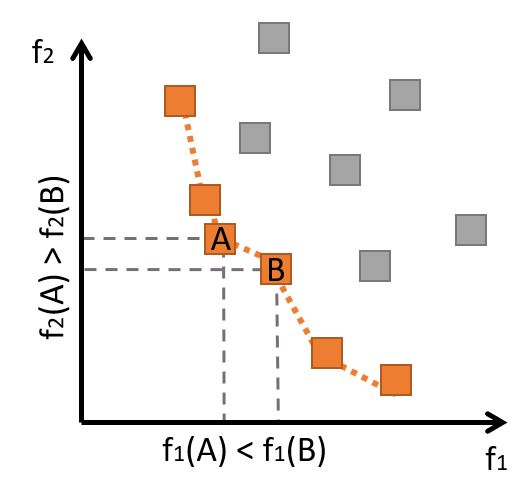
\includegraphics[width=5cm]{Images/Background/pareto-front.JPG}
		\caption[Representation of a Pareto front example for a bi-objective optimization problem]{Representation of the set of non-dominated (orange squares) and dominated (gray squares) solutions for a two-objective minimization problem. The Pareto front is composed of all the non-dominated solutions.}
		\label{fig:paretofrontier}
	\end{figure}
	% End Figure -------------------------------------------------------
	
	When considering the architectural practice, building design is a complex task that frequently involves dealing with multiple conflicting objectives, such as maximum lighting comfort \textit{versus} maximum thermal comfort, or minimum energy consumption \textit{versus} maximum thermal comfort. Even though the three previous approaches provide enough mechanisms for handling \ac{MOO} problems, they lack a more guided and informative strategy capable of retrieving a diverse and representative set of different trade-offs between the various performance aspects, i.e., the objective functions.
	
	Alternatively, the Pareto-based optimization approach provides the user with the set of non-dominated solutions that represent the different conflicts or trade-offs between the considered objectives. When confronted with this set of solutions, architects can compare the different design options, according to different performance criteria, and, thus, make more informed decisions about the different compromises involved. 
	
	On the other hand, in this approach, (1) the number of function evaluations is larger due to the need to find a set of optimal solutions instead of focusing on a single one, (2) the visual representation of the solutions’ objectives values becomes problematic when the number of objectives is greater than three, and (3) the way the optimization problem is modeled has a direct impact on the quality of the solutions.
	
	% #############################################################################
	
	\subsection{Comparison}
	\todo{Organizar tabela de forma mais lógica... O texto também...}
	
	This section focus on the comparison of the previously mentioned approaches, for which \Cref{table:optimization-approaches} provides a summarized view.
	
	\todo{Put column DoE before the SOO}
	\begin{table}[]
		\centering
		\resizebox{\textwidth}{!}{%
			\begin{tabular}{l|l|l|l|l|}
				\cline{2-5}
				& \multicolumn{1}{c|}{\begin{tabular}[c]{@{}c@{}}Single-objective \\ optimization\end{tabular}} & \multicolumn{1}{c|}{\begin{tabular}[c]{@{}c@{}}A priori preference \\ articulation\end{tabular}} & \multicolumn{1}{c|}{\begin{tabular}[c]{@{}c@{}}Pareto-based \\ optimization\end{tabular}} & \multicolumn{1}{c|}{\begin{tabular}[c]{@{}c@{}}Design of \\ experiments\end{tabular}} \\ \hline
				\multicolumn{1}{|l|}{Fundamentals} & \multirow{2}{*}{\begin{tabular}[c]{@{}l@{}}Maximization / \\ minimization\end{tabular}} & \multirow{2}{*}{Preferences} & \multirow{2}{*}{Pareto Front} & \multirow{2}{*}{Sampling} \\
				\multicolumn{1}{|l|}{} &  &  &  &  \\ \hline
				\multicolumn{1}{|l|}{Manual intervention} & \multirow{2}{*}{None} & \multirow{2}{*}{\begin{tabular}[c]{@{}l@{}}Preferences definition \\ (a priori)\end{tabular}} & \multirow{2}{*}{\begin{tabular}[c]{@{}l@{}}Preferences definition \\ (a posteriori)\end{tabular}} & \multirow{2}{*}{Constant} \\
				\multicolumn{1}{|l|}{} &  &  &  &  \\ \hline
				\multicolumn{1}{|l|}{Optimal solutions} & \multirow{2}{*}{Maximal / Minimal} & \multirow{2}{*}{Utility-based} & \multirow{2}{*}{Pareto optimal} & \multirow{2}{*}{Any} \\
				\multicolumn{1}{|l|}{} &  &  &  &  \\ \hline
				\multicolumn{1}{|l|}{Number of optima} & \multirow{2}{*}{1} & \multirow{2}{*}{1} & \multirow{2}{*}{1+} & \multirow{2}{*}{Unknown} \\
				\multicolumn{1}{|l|}{} &  &  &  &  \\ \hline
				\multicolumn{1}{|l|}{Provided information} & \multirow{2}{*}{Best solution} & \multirow{2}{*}{Best solution} & \multirow{2}{*}{Optimal solutions} & \multirow{2}{*}{Evaluated solutions} \\
				\multicolumn{1}{|l|}{} &  &  &  &  \\ \hline
				\multicolumn{1}{|l|}{Time Complexity} & \multirow{2}{*}{++} & \multirow{2}{*}{+++} & \multirow{2}{*}{+++++} & \multirow{2}{*}{+} \\
				\multicolumn{1}{|l|}{} &  &  &  &  \\ \hline
				\multicolumn{1}{|l|}{Configurable in process} & \multirow{2}{*}{Nothing} & \multirow{2}{*}{Preferences} & \multirow{2}{*}{Nothing} & \multirow{2}{*}{All} \\
				\multicolumn{1}{|l|}{} &  &  &  &  \\ \hline
				\multicolumn{1}{|l|}{Ease of use} & \multirow{2}{*}{+++} & \multirow{2}{*}{++} & \multirow{2}{*}{+} & \multirow{2}{*}{+++} \\
				\multicolumn{1}{|l|}{} &  &  &  &  \\ \hline
				\multicolumn{1}{|l|}{Ease of comprehension} & \multirow{2}{*}{Difficult} & \multirow{2}{*}{Difficult} & \multirow{2}{*}{Accessible} & \multirow{2}{*}{Easy} \\
				\multicolumn{1}{|l|}{} &  &  &  &  \\ \hline
				\multicolumn{1}{|l|}{Support in architecture} & \multirow{2}{*}{++} & \multirow{2}{*}{++} & \multirow{2}{*}{+} & \multirow{2}{*}{+++} \\
				\multicolumn{1}{|l|}{} &  &  &  &  \\ \hline
				\multicolumn{1}{|l|}{Main advantages} & \multirow{2}{*}{Time complexity} & \multirow{2}{*}{\begin{tabular}[c]{@{}l@{}}Search guided \\ towards a single objective\end{tabular}} & \multirow{2}{*}{\begin{tabular}[c]{@{}l@{}}Obtain different \\ trade-offs\end{tabular}} & \multirow{2}{*}{Full control} \\
				\multicolumn{1}{|l|}{} &  &  &  &  \\ \hline
				\multicolumn{1}{|l|}{Main Disadvantages} & \multirow{2}{*}{Lack of information} & \multirow{2}{*}{Lack of information} & Time complexity & Manual intervention \\
				\multicolumn{1}{|l|}{} &  &  & Results representation & No optima guarantees \\ \hline
			\end{tabular}%
		}
		\caption{Comparison between different optimization approaches}
		\label{table:optimization-approaches}
	\end{table}
	
	On the one hand, in terms of manual intervention, the design of experiments approach confers higher levels of control at the cost of constant manual intervetion (e.g., number of variations to generate, number of iterations to run sampling methods, choice of optimal solutions). The same does not happen with other approaches for which intervention is residual or even inexistent.	
	
	On the other hand, with higher control levels, the user gains more insight about the optimization process. Concretely, when following a design of experiments approach, the user is provided with all the information about all the solutions that were evaluated during the optimization process, whereas in the other approaches the user is only provided with the optimal solutions. The availability of information has a direct impact in the ability to comprehend the optimization results.
	
	The automation of optimization processes prompts the need for automatically evaluating the quality of solutions, thus requiring some optimality concepts: (1) depending on whether it is a maximization or a minimization problem, the \ac{SOO} approach considers the best solution to be the one presenting the largest or smallest value, respectively; (2) the \textit{a priori} preference of articulations approach applys a similar criteria, but it first entails the definition of a utility function to reduce a \ac{MOO} to a \ac{SOO} problem; and (3) the Pareto-based optimization approach is based on the Pareto optimality, leaving the final decision about the optimal solutions to the user.
	
	Depending on the approach, the solution's number and quality may vary. In general, all but the design of experiments approach presents a guided and, thus, more intelligent strategy to seek for efficient solutions. As a result, this approach does not guarantee that good solutions are found. Conversely, the other approaches tend to yield one or more optimal (or near) optimal solutions depending on whether it is a Pareto-based approach or not.
	
	A crucial point to take into consideration is the time difference between each approach, with the Pareto-based and the design of experiments approaches being the most and the less time-consuming, respectively. The former one requires searching the solution in space with the aim of finding the best trade-offs between different objectives, whereas the latter simply relies on a sampling strategy which generates different paramters' variations to be evaluated. This time difference is particularly concerning in the case of problems with costly evaluation functions, as it is the case of building design. Even though the \textit{a priori} preference-based approach involves the same objectives as the analogous Pareto one, it can be considerably faster. This results from the fact that this approach focus on the satisfiability of a certain set of preferences, instead of exploring a wider set of solutions.
	
	Indeed, when shifting to architecture, Pareto-based approaches are less applied in practice. Nevertheless, a few studies concerning this optimization approach have emerged in the past years, evidencing its utility~\cite{Evins2013,Hamdy2016}. Additionally, recent works show that despite the lower time complexity of \ac{SOO}-based and \textit{a priori} preference-based approaches, they are not as desirable as the Pareto-based ones~\cite{Attia2013,Cichocka2017SURVEY}. In fact, the latter ones enhance the decision making process, providing a clear insight about the trade-offs between the objectives involved. %Moreover, these multiple compromises represent different articulation of preferences from which the architect selects one. This approach is also called \textit{a posteriori} articulation of preferences.

	Despite the relevance and growing interest of Pareto-based optimization approaches, the lack of relevant benchmarks comparing the performance of different algorithms in the architectural field is evident. 

	\todo{Ease this transition...}Each optimization approach comprises different optimization algorithms. In the particular case of building design, the nature of the costly evaluation functions not only directly influences the overall optimization time, but also the algorithms' nature, as it will be discussed in the next section. 
	

% ##########################################################################
% ##########################################################################
% ##########################################################################
\section{Optimization Algorithms}
\label{sec:optimizationalgorithms}
	
	We have said that optimization processes are comprised by two parts: the first one, described previously, focused on the modeling of the problem and, a second one, which involves exploring the optimization model with the aim of finding more efficient solutions. This exploration part is achieved by means of optimization algorithms and will be the focus of this section. 
	
	Optimization algorithms search for the optimal solutions among the set of all possible solutions, called the solution space. Each algorithm implements different mechanisms and applies different types of information and techniques to enhance its search process in the solution space. This variety yields algorithms that are capable of addressing some partIcular type of problems very efficiently. that can solve some problems more or less efficiently than others algorithms~\cite{Wolpert1997NFLT}.
	
	In order to compare and identify which algorithms are more efficient, it is necessary to measure their quality and, whereas this is rather straightforward for \ac{SOO} algorithms, the same does not happen for \ac{MOO} algorithms, as it will be discussed in \Cref{ssec:performance}.
	
	\subsection{Algorithms Classification}
	\todo{Suavizar transição, falar do caso da arquitetura, dar uma ideia do que este capitulo vai falar}
	
	One important classification is regarding the strategies used to search for optimal solutions, particularly, with regards to the search aims of that strategy. Depending on the extent of the search, algorithms can be \textbf{global} or \textbf{local}. Local optimization algorithms strive to find a locally optimal solution, i.e., for which its value is better than all the other points in its vicinity. Moreover, local algorithms are usually highly sensitive to the starting point of the search and they tend to focus on smaller regions of the solution space. In contrast, global optimization algorithms strive to find globally optimal solutions, i.e., the best of all the locally optimal solutions. Global optimization algorithms explore larger regions of the solution space and frequently yield less precise results than the local ones.
		
	The second, and final, distinction is between \textbf{derivative-based} and \textbf{derivative-free} algorithms, which differ in the type of information used during the search for more efficient solutions. Derivative-based (or gradient-based) algorithms explore information from the derivatives of objective functions to guide the search. Consequently, they solve problems explicitly defined through mathematical forms very efficiently, as the derivatives' information is easily available. However, when neither the mathematical form, nor the information about the derivatives is easily available, it becomes necessary to explore other classes of algorithms. One example of such class is the derivative-free. Because derivative-free algorithms do not exploit any information about derivatives to guide the search for optimal solutions, they are remarkably suitable for addressing problems where information about the derivatives is impossible or impractical to obtain (e.g., the objective function's analytical form is unknown, time-consuming evaluations make information about the derivatives impractical to obtain). Instead, in order to find optimal solutions, derivative-free algorithms treat the objective functions as \textit{black-boxes} and use the result of previously evaluated solutions to guide the search~\cite{Rios2013}.\todo{Confirmar q/ derivative-free só serve pa isto... Vocabulário pode ter tornado o texto um pouco redutor}
	
	This last distinction is particularly relevant for the \ac{BPO} practice, since it is often impossible to attain a mathematical form for the objective functions, especially for complex designs. Alternatively, architects can use the results of performance simulation tools as the functions to optimize, thus replacing the closed-form mathematical expressions that relate design's parameters to the objective functions~\cite{Wortmann2016BBO}. Unfortunately, each simulation comprises a time-consuming task that may take up to seconds, minutes, hours, or even days to complete. As a result, derivative-based algorithms are not adequate solvers for these type of problems, as they would require an excessive amount of computational resources to collect the information about the derivatives. Instead, this information unavailability prompts the need for algorithms that treat such functions as \textit{black-boxes}, i.e., functions for which the algorithm has no information. A simple approach is to follow a design of experiments approach (as discussed \Cref{ssec:doe}) and systematically experiment with different parameter values until the best solutions are found. However, despite its inherent simplicity, that approach has several limitations, namely the fact that the its search strategies are uninformed and, consequently, require hundreds or thousands of iterations to converge to optimal solutions, which is not feasible when addressing problems with expensive evaluation functions. In the next section we discuss a second, and more complex, approach - the derivative-free optimization algorithms\footnote{These algorithms are also commonly known as black-box optimization algorithms within the architectural community~\cite{Wortmann2016BBO}}.
	
	% #############################################################################
	\subsection{Derivative-Free Optimization}
	\label{sec:dfo}
	 
	Derivative-free optimization algorithms do not use objective functions' information to seek for optimal solutions. Instead, they treat each objective function as a \textit{black-box}, for which it has no information about, and use the results of previous evaluations to guide the search towards the optimal solutions. \todo{Confirmar Luis and Sahidinis - definição e pôr referencia}
	 
	In the particular case of \ac{BPO}, derivative-free algorithms are able to overcome the difficulty of deriving analytical forms that emerges with the increase of building design's complexity~\cite{Machairas2014}. To this end, these algorithms treat the results of the performance simulations tools as the functions to optimize. The relevance of these algorithms' for design optimization is evident and translates into the multiplicity of studies that use them to optimize building designs' manifold aspects, including, among others, structural, lighting, thermal, energy consumption, and carbon-emissions \cite{Evins2011,Evins2012MOO,Evins2013, Wortmann2015AdvSBO,Wortmann2016BBO,Wortmann2017GABESTCHOICE,Wortmann2017Opossum,Waibel2018}. 
	
	For the past decades, the constant development and improvement of derivative-free optimization algorithms fostered the creation of algorithms with different properties and underlying assumptions. Although there is no standardized classification for these optimization algorithms~\cite{Rios2013, Wortmann2017ADO}, it is possible to group them differently according to their main mechanisms and ideas. This dissertation follows the classifications proposed by Wortmann in the context of architectural design~\cite{Wortmann2017ADO}. This classification first subdivides the algorithms in two groups according to the number of solutions generated in each iteration\todo{confirmar isto... What about simulated annealing?}, namely metaheuristics and iterative algorithms. Then, iterative algorithms are further subdivided into direct search and model-based algorithms, depending on the function that is explored during the search. Albeit the apparent chasm between these classifications, some algorithms draw ideas from distinct classes, thus emphasizing not only the blurred lines of such categorizations, but also the difficulties that lie with the definition of more standardized classifications. 
	
	The following sections describe each class and its intrinsic characteristics, proceeded by a brief comparison among them in light of the architectural design practice. 	
	
	% ----------- Subsection
	\subsubsection{Direct Search Algorithms}
	\label{ssec:direct-search}
	
	Although there seems to be no precise definition for direct search algorithms, these are often identified as algorithms that iteratively: (1) evaluate a finite sequence of candidate solutions, proposed by a simple deterministic strategy; and (2) select the best solution obtained up to that time~\cite{Kolda2003,Wortmann2016BBO}. Direct search algorithms are sought as valuable tools to address complex optimization problems, not only because most of them were proved to rely on solid mathematical principles, but also due to their good performance at initial stages of the search process~\cite{Rios2013}. 
	
	The main limitations of these algorithms is their performance deterioration with the increase on the number of input variables, and their slow asymptotic\todo{What about local algorithms in this class? Do they suffer from this as well?  Confirmar!} convergence rates as they become closer to the optimal solution~\cite{Kolda2003}. Moreover, literature review reveals that despite the existence of several algorithms and benchmarks comparing \ac{SOO} direct-search algorithms, only recently have these started to appear in the context of \ac{MOO}\todo{REF}. 
	
	Due to space issues, this dissertation opts for only providing the description of two representative algorithms of this class, referring \Cref{chapter:appendixA} to the reader for a more complete description of other direct search algorithms, including local algorithms, such as Nelder-Mead Simplex (NMS), SUBPLEX, and PRAXIS, a global algorithm called DIviding RECTangles (DIRECT), and a recently proposed \ac{MOO} algorithm known as Direct MultiSearch (DMS). In this section, we describe two representative algorithms in this class, which have been shown to be successful in the context of \ac{BPO}: NMS~\cite{Nelder1964} and DIRECT~\cite{Jones1993DIRECT}. 
	
	\todo{Adicionar mais detalhe... Está pobrezinho..}
	NMS is a local direct-search algorithm ...
	
	DIRECT is a global direct search algorithm that recursively subdivides the design space into smaller multidimensional hyper-rectangles, estimating the quality value of each rectangle. DIRECT uses these values to focus the search on more promising regions of the design space and to further subdivide those in smaller hyper-rectangles. 
	
	Overall, direct search algorithms are not as popular as other classes of derivative-free algorithms. Nevertheless, its convergence proofs and the recent developments in the field of \ac{MOO} make this class very appealing for \ac{BPO}. 
	
	% ----------- Subsection
	\subsubsection{Metaheuristics Algorithms}
	\label{ssec:metaheuristics}
	
	In the original definition, these algorithms were solely based in the interaction between local improvement procedures, called heuristics, and higher-level strategies, called metaheuristics. On the one hand, heuristics are techniques that locate good solutions, but not necessarily the optimal, nor the correct solution, and that often consider the trade-off between precision and quality, and computational effort. On the other hand, a metaheuristic is an algorithmic framework that can be applied to different problems, with a few modifications to add problem-specific knowledge, if so is desired~\cite{Glover2003Metaheuristics}. Moreover, a metaheuristic is a higher-level strategy that extends the capabilities of heuristics by combining one or more heuristic methods (referred to as procedures), while being agnostic to each heuristic. The ```meta'' classification of these algorithms results from the fact that they control the heuristics applied in the process.
	
	Throughout time, this class has grown to include any algorithm that includes simple heuristics to locate good solutions in complex design spaces, while considering the trade-off between precision, quality, and computational effort of the solutions. These algorithms often rely on randomization, and biological or physical analogies, to perform robust searches and to escape local optima~\cite{Glover2003Metaheuristics}. Additionally, their non-deterministic and inexact nature confers them the ability to effortlessly handle complex and irregular objective functions, as well as, to easily adapt to \ac{MOO} contexts, or even to provide domain-specific knowledge through the heuristics~\cite{Wortmann2017GABESTCHOICE}.
	
	Metaheuristics are efficient optimization algorithms when provided with sufficient amount of time to do the necessary objective function evaluations~\cite{Conn2009}. However, advantages can quickly become disadvantageous by simply changing the application context. This is the case of \ac{BPO} in the architectural practice, where each evaluation is a time-consuming task and the execution of thousands of evaluations rapidly becomes an infeasible scenario. Due to their stochastic nature, limiting the number of evaluations has severe repercussions, both on their convergence and performance guarantees~\cite{Hasancebi2009}. 
	
	Some of the most relevant metaheuristics algorithms include \ac{PSO} and \ac{EA} algorithms, like the \ac{GA}. We refer \Cref{chapter:appendixA} to the interested reader for more details about this and other metaheuristics algorithms.
	
	\todo{Melhorar substancialmente... Está demasiado genérico...}
	The single-objective \ac{PSO} algorithm\todo{ref} is a global metaheuristic algorithm inspired by biological systems, such as the collective behavior of flocking birds or fish schooling, which interact and learn from one another to solve problems~\cite{Brownlee2011}. In \ac{PSO}, the intelligence is decentralized, self-organized, and distributed throughout the participating particles, also known as swarm. These particles maintain information about their velocity, their current and personal best positions, and also the global best position known to the swarm. At each time step, the position and velocity of each particle are updated according to the best swarm or close neighbor position~\cite{Brownlee2011}.
	
	As \acp{EA}, \acp{GA} explore Darwinian natural selection concepts, such as heredity, reproduction, and natural selection, and genetics concepts and mechanisms, including genes, chromosomes, recombination, crossover, and mutation, in order to search for better solutions in the solution space. More concretely, \acp{GA} generate an initial random set of solutions, called population, which is then iteratively evolved, creating new generations. The evolution process is comprised of four main phases: (1) adaptability, where individuals of the population are assigned a suitability or fitness value; (2) selection, where pairs of individuals are selected for reproduction, based on a probabilistic function which is proportional to each individual's fitness value; (3) crossover, where the genotypes of the selected individuals are recombined to produce new individuals; and (4) mutation, where new individuals are subjected to random copying errors with a certain probability. While earlier generations are usually diverse, final generations are often very similar to the fittest individuals, i.e., we observe an intensification of the traits of the most suitable individuals, thus emulating the mechanism of natural selection, described by Darwin \cite{Brownlee2011}. % Besides genetic algorithms \cite{Golberg1989,Holland1992}, evolutionary algorithms encompass other algorithms such as Genetic Programming~\cite{Koza1992}, Evolution Strategies \cite{Schwefel1981}, Differential Evolution \cite{Storn1997}, among others. 
	
	Similarly to \acp{EA}, \acp{MOEA} adopt the evolutionary principles previously discussed, but have an additional archive to store the non-dominated solutions found~\cite{Zitzler2001SPEA2}. The archive technique is incorporated to prevent losing current non-dominated solutions due to random mutations or recombinations. Most \acp{MOEA} differ in the selection and reproduction operators used to iteratively evolve populations. These differences are usually related to the very own goals of approximating the Pareto front: (1) maximize the accuracy of the approximation (by minimizing the distance to the optimal front) and (2) maximize the diversity of the solutions in the front. While the first goal is related to the search strategy and how to assign fitness values in such a way that the individuals selected for offspring production will be closer to the Pareto-optimal front, the second goal is related to the time and storage constrains of the evolution process and which individuals to keep in each generation~\cite{Zitzler2001SPEA2}.
	
	Most modern \acp{MOEA} realize the accuracy and diversity ideas through some implementation of the following mechanisms~\cite{Zitzler2001SPEA2}:	
	\begin{itemize}
		\item Selection (or environmental selection): Besides the population, most \acp{MOEA} maintain an archive with the non-dominated front among all the solutions that were evaluated. The archive preserves individuals during several generations, only removing them if (1) a new solution is found to dominate them, or (2) if the archive size is exceeded and they happen to be in crowded regions of the front.
		
		\item Reproduction (or mating selection): At each generation, individuals are evaluated in two stages. The first stage compares them regarding the relation of Pareto dominance, using this information to define a ranking among these individuals. The second stage refines these rankings through the incorporation of density information, i.e., if the individuals lie in crowded regions.
	\end{itemize}
	
	These mechanisms can be completely indifferent from one another, e.g., the first one applying a Pareto-based criteria and the second one applying weighting approach. However, many \acp{MOEA} implement both concepts similarly. In the particular case of \ac{SPEA2}, the algorithm explores two independent sets of individuals: the population and the archive. In this algorithm, the archive size is fixed and, therefore, whenever the number of non-dominated individuals is less than its size, some dominated individuals are added to the archive. At each iteration, the algorithm computes each individual's fitness value (a \textit{strength} value, defined as terms of the number of solutions it dominates, the \textit{raw fitness} value, defined in terms of the strength of its dominators, and a density estimate, defined as the inverse of the distance to the $k^{th}$ to the nearest neighbor) and copies the non-dominated individuals from the population to the archive, removing any individual that is dominated, whose objective values are duplicated, or that, when the size of the updated archive is exceeded, lies in crowded regions of the non-dominated front. After filling the archive, pairs of individuals are chosen from the archive to reproduce and produce the offspring through recombination and mutation operators that will make the population of the next generation~\cite{Zitzler2001SPEA2}.
	
	As a \ac{MOEA}, \ac{NSGA-II} attempts to achieve an approximation to the Pareto front that is both accurate and diverse. In this particular algorithm, both the selection and reproduction mechanisms rely on the same basis criteria: Pareto dominance relations and a crowding measure. To define the order among the individuals, the pool of individuals is split into different Pareto fronts and ranked accordingly, i.e., the first non-dominated front is assigned the highest rank, the second front is assigned the second highest rank, and so on. Each individual in each rank is ordered according to a crowding measure, represented in terms of the sum of distances to the two closest individuals along each objective. The archive and the generation's population are combined, deleting the worst 50\%. Afterwards, binary tournaments are carried out on the remaining individuals (the archive members) in order to generate the next offspring population.	
	
	Overall, metaheuristics are random algorithms with no convergence guarantees, usually requiring several hundreds or even thousands of evaluations in order to obtain good solutions. For problems involving expensive evaluation functions, like building design, this algorithms are usually not a good choice. The overall time complexity of these algorithms becomes even more preoccupying in the case of \ac{MOO}, as the number of objectives raises.  Unfortunately, there is a predominance of these algorithms (e.g., \ac{GA}, \ac{SPEA2}, \ac{NSGA-II}) among \ac{BPO} practitioners, with very few tools providing support to other classes of algorithms. Nevertheless, these algorithms present several parameters that can be fine-tuned to improve their efficiency and, in fact, they can be very efficient solvers when configured properly. However, the optimal set of parameters is problem-specific and the same configuration applied to another problem might yield very bad performance.
	
	\subsubsection{Model-based Algorithms}
	\label{ssec:model-based}
	
	Model-based algorithms are effective handlers for time-consuming problems, where sensitive information is expensive to collect~\cite{Forrester2009SBO}. These problems are characterized by the large time complexity associated with the computation of the values of the objective function, and by the absence of previous knowledge about the objective function. Model-based algorithms are able to provide instant estimates of a design’s performance, by supplementing or replacing the original objective function by its approximation~\cite{Wortmann2016BBO}. This approximation, called the surrogate, is generated from a set of known objective function values and is then explored to determine the promising candidate solutions to evaluate next. The candidate solutions are then used to improve the surrogate and this process is repeated until a stopping condition is satisfied~\cite{Koziel2011}.
	
	Despite having a well-defined analytical form, which makes computations on the surrogate model more efficient than on the original objective function, the surrogate is only an approximate representation of the original function, and, therefore, must be constantly updated to guarantee a reasonable locally accurate representation~\cite{Koziel2011}. \Cref{fig:sbosexample} illustrates a surrogate that is accurate near the initial solutions. However, as we analyse solutions far from the initial ones, the accuracy of the surrogate model worsens.
	
	% Begin Figure: SBO Simple Example ----------------------------
	\begin{figure}
		\centering
		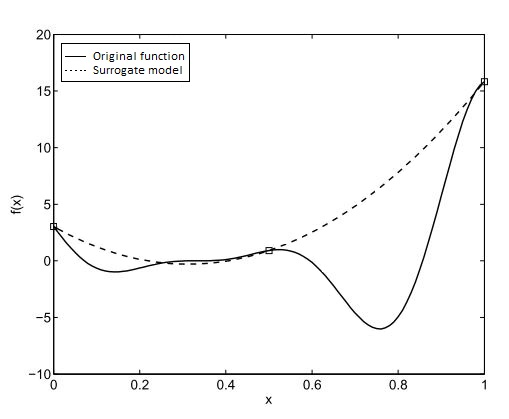
\includegraphics[width=8cm]{Images/Background/sbosexample.JPG}
		\caption[Example of a surrogate model]{Original function and corresponding surrogate model, created based on three initial solutions (squares). This image was retrieved from~\cite{Koziel2011}.}
		\label{fig:sbosexample}
	\end{figure}
	% End Figure -------------------------------------------------------
	
	Nowadays, the existing plethora of techniques applicable to the generation of surrogate models range from trust-region methods to \ac{ML} techniques. These techniques can be used to create (1) local surrogates, i.e., models where the approximation to the objective function is built around a certain point, and (2) global surrogates, i.e, models where the approximation is generated from all the obtained points. Whilst the former relies on the construction of simple, partial models of the objective function, the latter relies on the creation of a full model. The creation of the full model, requires balancing the need for improving the accuracy of the model by exploring broader regions in the solution space, with the need for improving the value of the objective function by exploiting promising regions~\cite{Koziel2011}. This balance is determined by a strategy that selects the next promising solution to evaluate.
	
	Undoubtedly, the best feature of model-based algorithms is the reduction in the total optimization time. This is particularly relevant in the context of \ac{BPO}, where each simulation may take seconds, minutes, hours, or even days to complete. However, the lower availability and the lack of necessary technical knowledge to implement or incorporate these algorithms into optimization processes are still obstacles to a broader adoption of this approach. Notwithstanding the existence of different studies involving \ac{ML} techniques for the creation of full surrogate models~\cite{Koziel2011, Forrester2009SBO}, such as neural networks, support vector machines, Radial Basis Functions (RBFs), and random forests, among others, only a few have actually been applied in the context of architecture. This scenario is even more self-evident when we shift from the single- to multi-objective optimization context.
	
	Two relevant local model-based implementations are the Constrained Optimization BY Linear Approximation (COBYLA) algorithm~\cite{Powell1994COBYLA}, and the Bound Optimization BY Quadratic Approximation (BOBYQA) algorithm~\cite{Powell2009BOBYQA}, that rely on the construction of simple, partial models of the objective function~\cite{Koziel2011}. The former uses the concept of a simplex to iteratively generate linear approximations of the objective function, whereas the latter generates quadratic approximations instead. 
	
	One relevant global model-based technique uses RBFs to create global approximations of the objective function. These approximations are simply the weighted sum of other, simpler, real-valued functions, the radial functions. These functions are defined on the Euclidean space $\mathbb{R}^n$ and their value depends on the distance to a center $c$, so that $\phi(x, c) = \phi(\left\lVert x-c \right\rVert)$. In an RBF technique, the weights are estimated based on the interpolation of data. A comprehensive detailed explanation of the RBF's estimation process is provided in~\cite{Forrester2009SBO}. 
	
	Overall, model-based algorithms are techniques that enable the creation of approximations of original functions and that usually uses other algorithms, like \acp{GA}, \acp{MOEA}, or even sampling algorithms. Particularly, global model-based algorithms exhibit very good performance at initial stages of an optimization process, especially when compared with metaheuristics. For these reasons, model-based algorithms are very appealing for problems involving costly evaluation functions, including \ac{BPO}'s problems.
	
	% ----------- 
	\subsubsection{Comparison}
	\label{ssec:comparisondfo}
	
	This section compares the different classes of derivative-free optimization algorithms mentioned in this chapter. \Cref{table:compare-dfo-algos} presents a summarized view of the main properties of these classes and, in the following paragraphs we compare them regarding their applicability in architecture. 

	% Please add the following required packages to your document preamble:
	% \usepackage{multirow}
	% \usepackage{graphicx}
	\begin{table}[]
		\centering
		\resizebox{\textwidth}{!}{%
			\begin{tabular}{r|c|c|c|}
				\cline{2-4}
				& Direct search & Metaheuristic & Model-based \\ \hline
				\multicolumn{1}{|r|}{Main Mechanism / Strategy} & \begin{tabular}[c]{@{}c@{}}Sequential evaluation of \\ candidate designs\end{tabular} & \begin{tabular}[c]{@{}c@{}}Combine and randomly modify \\ previous known best designs\end{tabular} & \begin{tabular}[c]{@{}c@{}}Optimize a secondary model, \\ instead of the expensive one\end{tabular} \\ \hline
				\multicolumn{1}{|r|}{Deterministic} & Yes & No & Yes \\ \hline
				\multicolumn{1}{|r|}{Convergence guarantees} & Yes & No & Sometimes \\ \hline
				\multicolumn{1}{|r|}{Convergence rate (evals)} & Early (100-300) & Late (typically \textgreater{}1000) & Early (100-300) \\ \hline
				\multicolumn{1}{|r|}{Number of solutions} & 1 & More than 1 & 1 \\ \hline
				\multicolumn{1}{|r|}{Applicability to MOO} & Extremely rare & Very frequent & Unusual \\ \hline
				\multicolumn{1}{|r|}{Ease of use} & + & ++ & + \\ \hline
				\multicolumn{1}{|r|}{Ease of implementation} & + & +++ & + \\ \hline
				\multicolumn{1}{|r|}{Support in architecture} & + & +++ & + \\ \hline
				\multicolumn{1}{|r|}{\multirow{2}{*}{Main advantages}} & Deterministic & Applicable to any domain & Time complexity decrease \\
				\multicolumn{1}{|r|}{} & Convergence rate & Flexible & Convergence rate \\ \hline
				\multicolumn{1}{|r|}{\multirow{2}{*}{Main disadvantages}} & \multirow{2}{*}{\begin{tabular}[c]{@{}c@{}}Time complexity grows exponentially \\ with the number of parameters\end{tabular}} & Low convergence rate & \multirow{2}{*}{\begin{tabular}[c]{@{}c@{}}Time complexity grows exponentially \\ with the number of parameters\end{tabular}} \\
				\multicolumn{1}{|r|}{} &  & No convergence guarantees &  \\ \hline
			\end{tabular}%
		}
		\caption{Comparison between the derivative-free algorithms' classes.}
		\label{table:compare-dfo-algos}
	\end{table}
	
	The multidisciplinary aspect of building design raises distinct problems, ranging from well-behaved problems with simple, unimodal, convex functions to more ill-behaved problems with irregular, multimodal objective functions~\cite{Wortmann2017ADO}. In addition to problem's diversity, the time complexity associated to function evaluations also becomes an important factor to consider, when pondering each category's impact on \ac{BPO} problems.
	
	The problems' plethora within performance-based design is vast: a specific optimization algorithm may perform well for some problems and have a terrible performance in other problems~\cite{Wortmann2017GABESTCHOICE, Fang2017}. This idea resembles the ones captured in Wolpert's \acp{NFLT} for optimization, which state that any algorithm's worse performance over some classes of problems offsets its better performance in other classes. Because of the distinct nature of architectural design problems, the arguments applied in architecture are not necessarily applicable to the other fields, like science and engineering. 
	
	Inevitably, the same building design description might yield different problem descriptions according to the performance aspects being considered. Some algorithms might explore certain descriptions more effectively than others, e.g., because the objective functions describing the lighting and structural behavior of a certain design may have completely different properties. In an attempt to exploit this property, \ac{BPO} practitioners often dedicate a small amount of their total time budget to test various algorithms and different setup parameters, before finally settling for an optimization algorithm~\cite{Hamdy2016}.	
	
	Regarding the different algorithms' categories, it is interesting to see the metaheuristics' popularity among researchers and practitioners. The main reasons behind the idolization of the metaheuristics are their (1) inherent simplicity, (2) ease of implementation, and (3) wide applicability to different domains~\cite{Wortmann2017ADO}. Unfortunately, other categories do not benefit from such properties, which is a limitation towards their application in architectural domains. Moreover, the lack of easy-to-use tools involving algorithms from other categories are also limiting their application in architectural contexts. Firstly, the existing non-metaheuristic tools are usually available as programming libraries, instead of being integrated in architectural design workflows. As a result, to use the optimization algorithms, architects often need some programming knowledge to create the scripts to integrate the algorithms into the design workflow. However, since architects typically lack the required knowledge, they tend to struggle with the scripts' production and, eventually, opt for using friendlier metaheuristics ready-to-use tools. Given this facts, it is not surprising that most of the existing building design optimization literature ends up focusing on the application of algorithms from the metaheuristics category~\cite{Hamdy2016,Nguyen2014,Evins2013}. 
	
	However, in the light of the \acp{NFLT}, the need for more short-term efficient optimization approaches fostered the development of tools exposing algorithms with different properties. Particularly, plug-ins like Goat~\cite{GOAT} and Opossum~\cite{Wortmann2017Opossum} enable the usage of algorithms from both direct search and model-based classes. These tools expose optimization algorithms from the NLopt~\cite{NLOPT} and RBFOpt~\cite{RBFOPT} frameworks, respectively, providing friendly, ready-to-use interfaces within Grasshopper~\cite{GRASSHOPPER}, a visual programming environment that enables the parametric design and performance evaluation of building designs for different values of the parameters. For the past few years, few works have compared different algorithms using these tools with the ones available in other metaheuristics tools (e.g., Galapagos~\cite{GALAPAGOS}, Octopus\cite{OCTOPUS}, Optimo~\cite{OPTIMO}, Silvereye~\cite{Cichocka2017SILVEREYE}).
	
	Although the results may vary, in general, direct search and surrogate-based algorithms seem to be more effective than the metaheuristics ones in initial stages of the optimization process~\cite{Wortmann2017,Wortmann2016BBO,Wortmann2017GABESTCHOICE}. Even some metaheuristics algorithms can be very effective approaches for some optimization problems~\cite{Waibel2018}. One can explore these performance fluctuations to find the most effective optimization algorithm for a specific problem. This performance gain can be determining in the overall optimization time, especially when complex and time-consuming simulations are involved. Indeed, several authors ~\cite{Wortmann2016BBO,Hamdy2016} suggest that the selection of the optimization algorithm should be based on the results of several tests with different methods for a fixed number of evaluations or a fixed amount of time. 
	
	Optimization is a useful tool to address both single and multi-objective problems. In architecture, most optimization applications focus on single-objective problems and cover the three different derivative-free algorithms classes. However, the same does not happen with multi-objective problems, with only one of the classes being extensively applied to \ac{MOO} building design: the metaheuristics~\cite{Hamdy2016}. The main reason behind metaheuristics popularity is their broader adaptability to both varying degrees of complexity and to different problem domains~\cite{BlumRoli2003Metaheuristics}.
	
	Recent developments in multiple surrogate-assisted \acp{MOEA} in the fields of science and engineering~\cite{Zapotecas-Martinez2016,Hussein2016} made it possible to decrease the number of expensive evaluations in \ac{MOO} problems. Generally, these techniques combine metaheuristics methods, which find more than one solution within a single execution, with surrogate models, which are approximations of the original objective functions. Diaz-Manriquez et al.~\cite{Diaz-Manriquez2016} provide a comprehensive overview of surrogate-assisted techniques for \ac{MOO} from the engineering perspective. 
	
	The following sections focus on the current \ac{BPO} practices both for \ac{SOO} and \ac{MOO}, the currently available tools, and the advantages and disadvantages of each approach.
	
	\subsection{Performance Indicators}
	\label{ssec:performance}
	Despite the large interest in \ac{MOO}, the question of how to quantitatively compare the performance of different algorithms still remains unanswered. Firstly, in multi-objective problems, the number of objectives is greater than the number of objectives in single-objective problems: the former considers a collection of vectors representing the Pareto-optimal solutions, whereas the latter considers real numbers. Secondly, it is often the case that the application of exact methods to \ac{MOO} contexts is impracticable due to the complexity introduced by underlying applications (e.g., simulation tools, physical experiments). In these cases, the generation of the true Pareto-optimal set is often infeasible, requiring vast computational resources to be generated. Thirdly, despite the availability of alternatives to exact methods, such as metaheuristics algorithms (e.g., evolutionary algorithms, particle swarm), these are not guaranteed to identify optimal trade-offs, instead yielding good approximations~\cite{Zitzler2003Metrics}. Finally, we are interested in knowing which of the non-exact algorithms yields better approximations for a given problem, hence prompting the need for assessing the performance of \acp{MOOA}.
	
	The notion of performance includes not only the quality of the results, but also of the computational resources needed to generate such results. While the latter aspect is usually identical for both \ac{SOO} and \ac{MOO}, which either typically consider the number of expensive evaluations or the overall run-time on a particular computer, the quality aspect is considerably different. Because \acp{SOO} consider real-valued objective spaces, the quality is defined in terms of the objective function: the smaller (or larger) the value, the better the solution. However, \acp{MOO} consider vector-valued objective spaces, thus requiring another concepts like Pareto dominance. Unfortunately, when considering the Pareto dominance concept a few issues may arise, namely the possibility of two solutions being incomparable, i.e., when neither dominates the other, or having solutions in one set that either dominate or are incomparable to those in the other set of solutions and vice versa. 
	
	Literature review evidences the existing struggle to define the meaning of quality with respect to approximation of Pareto-optimal sets~\cite{Knowles2002Metrics,Riquelme2015}. However, the quality of Pareto sets is usually evaluated in terms of three aspects: (1) cardinality, meaning larger sets of solutions, (2) diversity, meaning that solutions should be as uniformly distributed as possible, so as to obtain a representative set of solutions covering to larger extents the different trade-offs, and (3) accuracy, meaning that solutions should be as close as possible to the true Pareto-optimal set or Pareto Front. 
	
	For the past decades, several indicators have been proposed to measure the quality of Pareto sets, ranging from unary quality measures, which assign each approximation set a number that reflects a certain quality aspect, to binary quality measures, which assign numbers to pairs of approximation sets, among others. This thesis considers a small but representative set of quantitative indicators to measure the quality of \acp{MOOA}' results with respect to the three aspects: cardinality, diversity, and accuracy. 
	
	Literature review reveals the existence of dozens of indicators that consider either one of the mentioned aspects or a combination of them. In the following definitions we use the term \textit{approximation set} to denote the Pareto Front returned by an optimization algorithm, and we use the term \textit{reference set} to denote the true Pareto Front or, whenever that is not possible, an estimate of the true Pareto front. 
	In this section, we list some of the most used indicators for assessing the performance of evolutionary \acp{MOO}~\cite{Riquelme2015}. 
	
	
	\subsubsection{Unary Indicators}
	% ---------------------------
	% Unary Indicators 
	% ---------------------------
	%% https://github.com/PastelBelem8/MscThesis/blob/metrics/src/indicators/MOOIndicators.jl
	% Cardinality 
	With regards to the cardinality aspect, there are essentially two indicators:
	\begin{itemize}
		\item \textbf{\ac{ONVG}} computes the number of non-dominated solutions in the approximation set ~\cite{Veldhuizen1999GD}.
		\item \textbf{\ac{ONVGR}} computes the ratio of non-dominated solutions in the approximation set with regards to a reference set~\cite{Veldhuizen1999GD}.
	\end{itemize}
	
	Cardinality indicators are based on the intuition that a good approximation set would have many optimal solutions. However, these indicators alone do not suffice to provide an accurate measure, as they privilege quantity over quality of solutions~\cite{Veldhuizen1999GD}, i.e., they often qualify approximation sets having dozens or hundreds of dominated solutions as being better than sets that provide fewer non-dominated solutions. This completely distorts the initial idea of finding the best Pareto front, i.e., set of non-dominated solutions.
	
	% || Diversity / Distribution ||
	To complement cardinality indicators, it is often advisable to consider the diversity aspect of approximation sets as well. A few well known diversity-based indicators are:
	\begin{itemize}
		\item  \textbf{Spacing} (or Set Spacing) computes the variance of the Manhattan distances between each non-dominated solution and its closest neighbor. It measures how well-spaced the solutions from the approximation set are. A value of zero represents equally spaced non-dominated solutions. 
		\item \textbf{Spread} (or $\Delta$) is similar to Spacing. However, it calculates the normalized variance and uses the Euclidean distance instead.
		\item \textbf{Maximum Spread} (or \textbf{$M_3^\ast$}) computes the Euclidean distance between the bounds of each objective dimension. It measures the extent of the objective space in each dimension by calculating the distance between the maximum and minimum of each objective. A greater value indicates larger coverage of the objective space.
		
		\item \textbf{Entropy} uses the Shannon's entropy concept to measure the uniformity of the approximation set distribution. This indicator makes the assumption that each solution provides some information about its vicinities, thus modeling each solution with Gaussian distributions. These distributions add up to form a density function capable of identifying peaks and valleys in the objective space, corresponding to dense and sparse zones, respectively. 
		
		\item \textbf{Diversity Metric} is similar to the Entropy indicator. However, it projects the solutions of both the approximation set and the reference set to an hyperplane which is subdivided uniformly. It assigns each interval two numbers: one number marking whether that interval contains at least one optimal solution in the reference set, and the second number marking whether the interval in addition to the optimal solution in the reference set, also contained at least one solution in the approximation set. Then, the diversity measure is the sum of the score of each interval, which are assigned using a sliding window technique (considering one interval and its immediate neighbors) based on the value of the marks\footnote{The scoring function considers the distribution of the marks in three consecutive grids. The function's proper definition can be found in \cite{Deb2002DM}.}. So, the diversity of the reference set considers the value of the first marks, whereas the diversity of the approximation set considers the values of the second marks. In the end, the diversity metric is given by the relative difference between the diversity of the approximation set and the diversity of the reference set. The best diversity possible is achieved if all intervals enclose at least one point\cite{Deb2002DM}.
		% Then, it computes the ratio between the number of intervals that have at least one non-dominated solution from both sets and the number of intervals that have at least one non-dominated solution of the reference set. Higher values of the diversity metric imply a better distribution and higher diversity of the approximation set when compared to the reference set itself. 
		
	\end{itemize}
	
	While these indicators are more robust, considering these indicators alone will not necessarily identify sets having Pareto optimal solutions, as they prioritize sets where solutions are spaced evenly apart or that cover broader regions of the objective space~\cite{Veldhuizen1999GD}. Moreover, because most of them assume that the Pareto front will be continuous, they may behave erroneously when facing problems with disconnected Pareto fronts. The diversity metric attempts to alleviate these limitations by comparing the non-dominated solutions of the approximation set with those of the reference set \cite{Deb2002DM}.
	
	% || Accuracy ||
	Previous metrics are not good indicators of how close the approximation sets really are to the reference set. To obtain a measure of the convergence of the results, one should consider accuracy indicators, such as:
	\begin{itemize}
		% ER
		\item \textbf{\ac{ER}} computes the proportion of false-positives in the approximation set, i.e., the ratio of optimal solutions in the approximation set that are not optimal in a given reference set~\cite{Veldhuizen1999GD}. Lower values of \ac{ER}, represent better approximation sets. 
		% MPFE
		\item \textbf{\ac{MPFE}} computes, for each solution in the approximation set, the minimum Euclidean distance to the closest solution in a given reference set, returning the maximum of those distances~\cite{Veldhuizen1999GD}. In other words, it returns the maximum error of the approximated Pareto Front. Lower values of \ac{MPFE} imply better approximation sets. 
		% Generational Distance
		\item \textbf{\ac{GD}} computes the average distance of an approximation set to a given reference set by computing the distance of the solutions in the approximation set to the nearest points in a given reference set averaged on the number of solutions in the approximation set~\cite{Veldhuizen1999GD}. A value of $0$ indicates that all the solutions in the approximation set are in the reference set. Different authors\cite{Zitzler2000m1m3} refer to this metric as \textbf{$M_1^\ast$}.
	\end{itemize}
	
	Accuracy indicators, like the previous indicators, can also produce misleading results and, therefore, should be considered together with other metrics. In general, all these three indicators have flaws, for instance, \ac{ER} focus on errors instead of focusing on the optimal solutions. As a result, it penalizes larger approximation sets that, despite having a more representative set of the real optimal solutions, have made more errors than other approximation sets with fewer solutions and, potentially, less errors. On the other hand, \ac{MPFE} focus on the maximum error of an optimal solution in the approximation set, when compared to the reference set. As a result, approximation sets, whose points are closer to the Pareto front but that have an outlier, will have higher values of \ac{MPFE} than other approximation sets, whose points are further away from the reference set but at a smaller distance than the outlier is from the reference set. At last, \ac{GD} has also been shown to behave erroneously, especially due to its dependency on the cardinality of the approximation set~\cite{Ishibuchi2005GDIGD}.
	
	The final set of indicators considers the accuracy and diversity aspects simultaneously:
	\begin{itemize}
		% Hypervolume
		\item \textbf{\ac{HV}} (or Lebesgue measure or S-metric) measures the size of the objective space covered by an approximation set, i.e., it measures the volume of the dominated space. It provides the unique and desirable properties of (i) Pareto \textit{compliance}, i.e., an approximation set which completely dominates another, will necessarily have a greater volume than the latter, and (ii) convergence guarantees, i.e., any approximation set that achieves the maximum possible volume is guaranteed to contain all Pareto-optimal solutions.
		% Inverted GD
		\item \textbf{\ac{IGD}} is the opposite of \ac{GD}, instead computing the average distance between a given reference set and the approximation set. \ac{IGD} computes the distances between each solution in the reference set and its closest solution in the approximation front, averaged over the size of the reference set. When the solutions in the reference set are well distributed, smaller values of \ac{IGD} suggest better and well-distributed approximation sets. Previous works have referred to this metric as \textbf{$D1_R$}~\cite{Ishibuchi2005GDIGD}\todo{Save REFs, a verdadeira ref está no Hansen1998}. 
	\end{itemize}
	
	Despite considering the diversity and accuracy aspects of Pareto fronts, \ac{IGD} is still Pareto non-compliant and has been shown to behave erroneously under certain conditions~\cite{Ishibuchi2005GDIGD}. Conversely, \ac{HV} is the only metric that exhibits the Pareto-compliance property. However, its usage is often impractical in problems, where the number of objectives is greater than ten, due to the its exponential grow with the number of objectives \cite{Ishibuchi2005GDIGD}.
	
	
	\subsubsection{Binary Indicators}
	In situations where the original Pareto-optimal set is not available, the binary indicators provide a way to compare approximation sets with respect to all the aspects. Among the most frequently used indicators, we emphasize:
	\begin{itemize}
		\item \textbf{Two set coverage} (or $C$) yields the number of solutions in one approximation set that are dominated by at least one of the solutions of the other approximation set. A value of $1$ suggests that the second approximation set is completely dominated by some solutions in the first one, whereas a value of $0$ represents the situation when none of the solutions of the second approximation set is covered by the first approximation set.
		
		\item \textbf{Epsilon Indicators} ($\epsilon$) that gives a factor by which an approximation set is worse than another considering all objectives, i.e., given two approximation sets $A$ and $B$, it computes the smallest amount $\epsilon$ by which $A$ must be translated, so that every solution in $B$ is dominated by at least one solution in $A$.
		
		\item \textbf{R-metrics} consider a family of indicators where the quality of each approximation set is defined according to a set of utility functions, and the larger the utility value of some set, the better the quality. R-metrics declare that the best approximation set will be the one that is better with regards to most utility functions:
		\begin{itemize}
			\item \textbf{$R1$} determines whether the an approximation set is better, equal, or worse than the other. 
			\item \textbf{$R2$} computes the expected mean difference in the utilities of both approximation sets.
			\item \textbf{$R3$} computes the expected mean relative difference in the utilities of both approximation sets.
		\end{itemize}
	\end{itemize}
	
	When comparing the usefulness of binary indicators, these usually aim at comparing different approximation sets and not necessarily the quality of the sets. This is the case of the two set coverage indicator, which allows to compare the existing Pareto-dominance relation between two sets, but does not allow to infer any other information (e.g., how worse one set is regarding the other). Moreover, this indicator becomes erroneous when the two sets are incomparable, i.e., neither dominates the other~\cite{Zitzler2003Metrics}. In contrast to the two set coverage indicator, the epsilon family indicators enable more informed comparison among two different approximation sets, as it provides a measure of the relative difference between the two sets. Finally, because the R-metrics incorporate utility functions, the user is able to introduce a preference over the objectives, thus influencing the optimality of each set. 
	
\section{Optimization in Architecture}	
	\label{sec:plugins}
	
	For years, multiple derivative-free optimization libraries have been developed (e.g., NLopt, RBOpt, Platypus, DEAP, Pyomo, PISA, jMetal, MOEAFramework). However, in order to use them within architectural practices, architects had to code the integration scripts to connect the simulation models for different variations of the parametric models and the optimization libraries\cite{Attia2013}. Moreover, these frameworks often lacked post-processing and visual features, which antagonized the readability and comprehension of the results~\cite{Attia2013,Nguyen2014}.
	
	Several plug-ins have been developed in an attempt to reduce the limitations associated to the coupling of simulation tools and mathematical optimization frameworks, thus providing a seamless connection between the parametric models produced in computational design tools, like \ac{CAD} and \ac{BIM} tools, the simulation or analytical models, and the optimization frameworks. Given the visual nature of architects, these plug-ins provide friendly, ready-to-use optimization interfaces, which are usually coupled with a few post-processing and visual features to enhance the intelligibility of optimization results. 
	
	Currently, existing optimization plug-ins are implemented on top of the visual parametric tools: Grasshopper~\cite{GRASSHOPPER} and Dynamo~\cite{DYNAMOBIM}. In \Cref{fig:opt-plugins}, we represent the most relevant optimization plug-ins among \ac{BPO} practitioners: Galapagos, Goat, Octopus, Opossum, and Silvereye implemented on top of Grasshopper, and Optimo implemented on top of Dynamo. In the following sections we briefly discuss each plug-in.
	
	% Begin Optimization Plug-ins Figure -------------------------------------------------------
	\begin{figure}
		\centering
		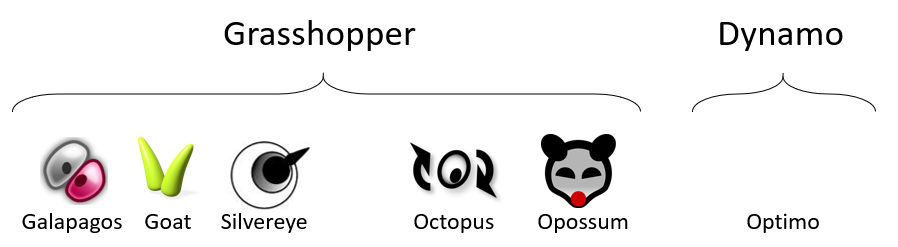
\includegraphics[width=\textwidth]{Images/Background/opt-plugins.PNG}
		\caption[Optimization Frameworks in the Architectural Practice]{Optimization frameworks currently used in architectural practices.}
		\label{fig:opt-plugins}
	\end{figure}
	% End Figure -------------------------------------------------------
	
	\subsection{Galapagos}
	\label{subsec:galapagos}
	% General description of Galapagos, intuition
	Galapagos~\cite{GALAPAGOS} is a generic plug-in, implemented on top of Grasshopper, designed to allow the application of metaheuristics algorithms by non-programmers to solve a wide variety of problems. 
	
	% Optimization Algorithms
	Particularly popular amongst architects~\cite{Wortmann2017ADO} for its \ac{GA}, Galapagos also provides other global metaheuristic solver, called simulated annealing (see \todo{referenciar secção dos algoritmos xD}). 
	
	% User Experience
	To use one of the solvers, architects must first define a script in using Grasshopper's components, such as sliders, values lists, area, distance, among others. This script should be organized in three distinct parts: (1) the Input, where they specify the design's parameters; (2) the Generation, where they create the design's algorithmic model that when instantiated with the parameters' values will generate the 3D model; and (3) the Analysis, where they define the analysis or objective function which they ought to optimize. 
	
	After creating the program script, the architect must drag the Galapagos' component to the script and connect it to the design parameters and to the objective function. Note, however, that Galapagos require the variables to be defined in terms of sliders components, interpreting their numerical range as the variables' lower and upper bounds, and the objective function to be output to a number component. The Galapagos' component refers to the variables as genome and to the objective function as fitness.
	
	Galapagos' \ac{GUI} is displayed upon double-clicking the Galapagos' component (see \Cref{fig:galapagosoptions}). The interface is simple, friendly, intuitive, and well-organized. Moreover, all options are filled by default, thus promoting a ready-to-use (or click-and-run) interaction, which makes it particularly easy to use by users with no experience or expertise in the field. Unfortunately, more experienced users might feel frustrated using this plug-in, as they are only able to modify a few parameters of the solver, thus lacking a finer control over the process. 
	
	In addition to not requiring any integration efforts or any programming-related knowledge to setup and use its capabilities, Galapagos also provides a visually rich experience, by providing different runtime graphical views of the optimization process. Galapagos supports different views depending on the optimization solver being used (see \Cref{fig:galapagosviewsa} and \Cref{fig:galapagosviewsb}):
	\begin{itemize}
		\item fitness graph that either represents the distribution of fitness values in the population discriminated by generations. Exhibited for both solvers;
		\item similarity representation graph that represents solutions that are genetically similar close to each other, and marks solutions that contribute to the creation of the next generation with black dots, whilst non-contributors are marked with a red cross. Exhibited for the \ac{GA} solver;
		\item vertical parallel coordinates graph, where each vertical line corresponds to a parameter, and solutions are represented as line segments connecting different parameters values. Exhibited for the \ac{GA} solver;
		\item ranked list of the best solutions found. Exhibited for both solvers;
		\item temperature graph, representing the temperature decrease rate of the simulated annealing process with each time step. Exhibited for the simulated annealing solver.
	\end{itemize}
	
	Overall, these views provide a visual feedback about the course of the optimization run and highlight the best solutions found up to that generation. In the end, the user is able to navigate through generations and re-instantiate these solutions in the corresponding \ac{CAD} tool, and, consequently to better understand the obtained results. Moreover, the ranked list of the results allow the user to select the one he appraises the most the amongst multiple optimal solutions found by the solver. Unfortunately, Galapagos lacks logging mechanisms which causes the information about the optimization enclosed within these views to be lost as soon as the \ac{GUI} is closed. 
	\begin{figure*}[htbp]
		\centering
		\subfigure[]{%
			\label{fig:galapagosoptions}%
			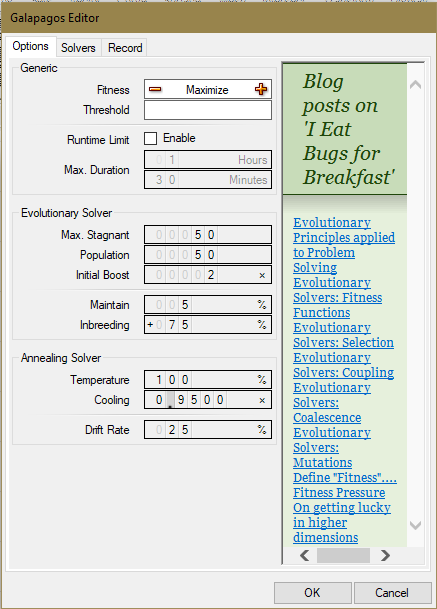
\includegraphics[width=0.30\textwidth]{Images/Background/Galapagos/Galapagos-algorithms-setup.PNG}}%
		\hfill
		\subfigure[]{%
			\label{fig:galapagosviewsa}%
			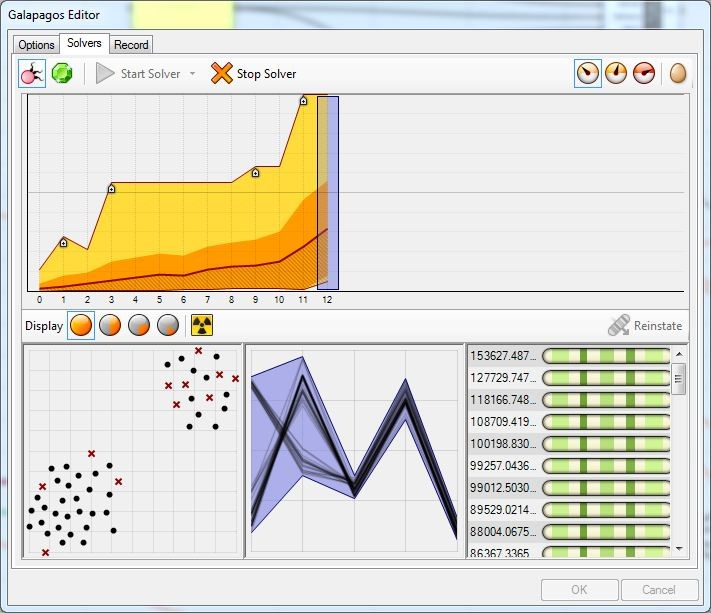
\includegraphics[width=0.345\textwidth]{Images/Background/Galapagos/galapagosvis.JPG}}%
		\hfill
		\subfigure[]{%
			\label{fig:galapagosviewsb}%
			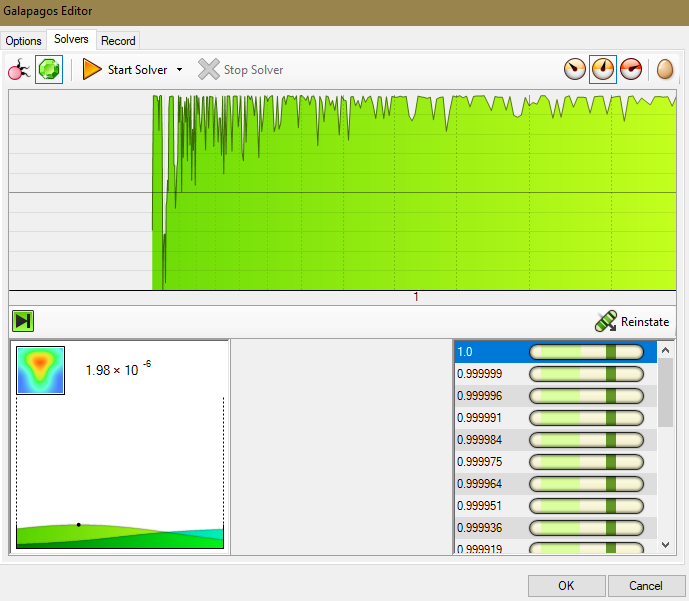
\includegraphics[width=0.345\textwidth]{Images/Background/Galapagos/galapagos-sa-results-2.PNG}}%
		
		\caption[Galapagos GUI]{ Three views of the Galapagos' \ac{GUI}: (a) Solvers configuration menu (b) Graphical views for the \ac{GA} solver (c) Graphical views for the simulated annealing solver}
		\label{fig:galapagos}
	\end{figure*}
	
	% ----------------- [GOAT] ------------------
	\subsection{Goat}
	% General description, intuition
	Goat \cite{GOAT} is a generic optimization plug-in, implemented on top of Grasshopper, designed to enable non-programmers to solve numerous problems.
	
	Unlike Galapagos, Goat interfaces the NLopt mathematical optimization library~\cite{NLOPT} to provide single-objective algorithms from all the derivative-free classes mentioned earlier (see \cref{sec:dfo}), including one global direct search (DIRECT), one local direct search (Subplex), one global metaheuristic (CRS2), and two local model-based algorithms (COBYLA and BOBYQA). 
	
	Goat is strongly influenced by Galapagos, also requiring a script in Grasshopper entailing the definition of the problem. In this script, the user drags the Goat's component to the script connecting it to the design parameters and the objective function, which, like Galapagos, must be sliders and number components, respectively (see \Cref{fig:goat}).
	
	Goat's \ac{GUI} is displayed after double-clicking the Goat's component (see \Cref{fig:goat}). This interface comprises a single menu, which is simple and straightforward to use. Like Galapagos, Goat is also distributed in a ready-to-use format with all the extra configuration parameters' values filled by default. As a result, non-programmers can easily explore this tool to address complex problems. Unfortunately, Goat provides no options for a more experienced user to configure the algorithms, except to configure the initial point of the search.
	
	Despite requiring no additional efforts to use Goat's optimization capabilities, the absence of visual and interactive mechanisms severely hinders the reputation of Goat. Firstly, it provides no visual feedback (e.g., solution lists, plots) about the course of the optimization run. Secondly, it also does not create log files to monitor the optimization process. Thirdly, the user is not able to interact with the optimization process. Finally, it returns a single optimal solution, whose values are represented in the sliders and number components. All these reasons contribute to a non-informed and non-traceable optimization process that inspires no confidence it the attained results. 
	
	% Begin Goat-Options Figure -------------------------------------------------------
	\begin{figure}
		\centering
		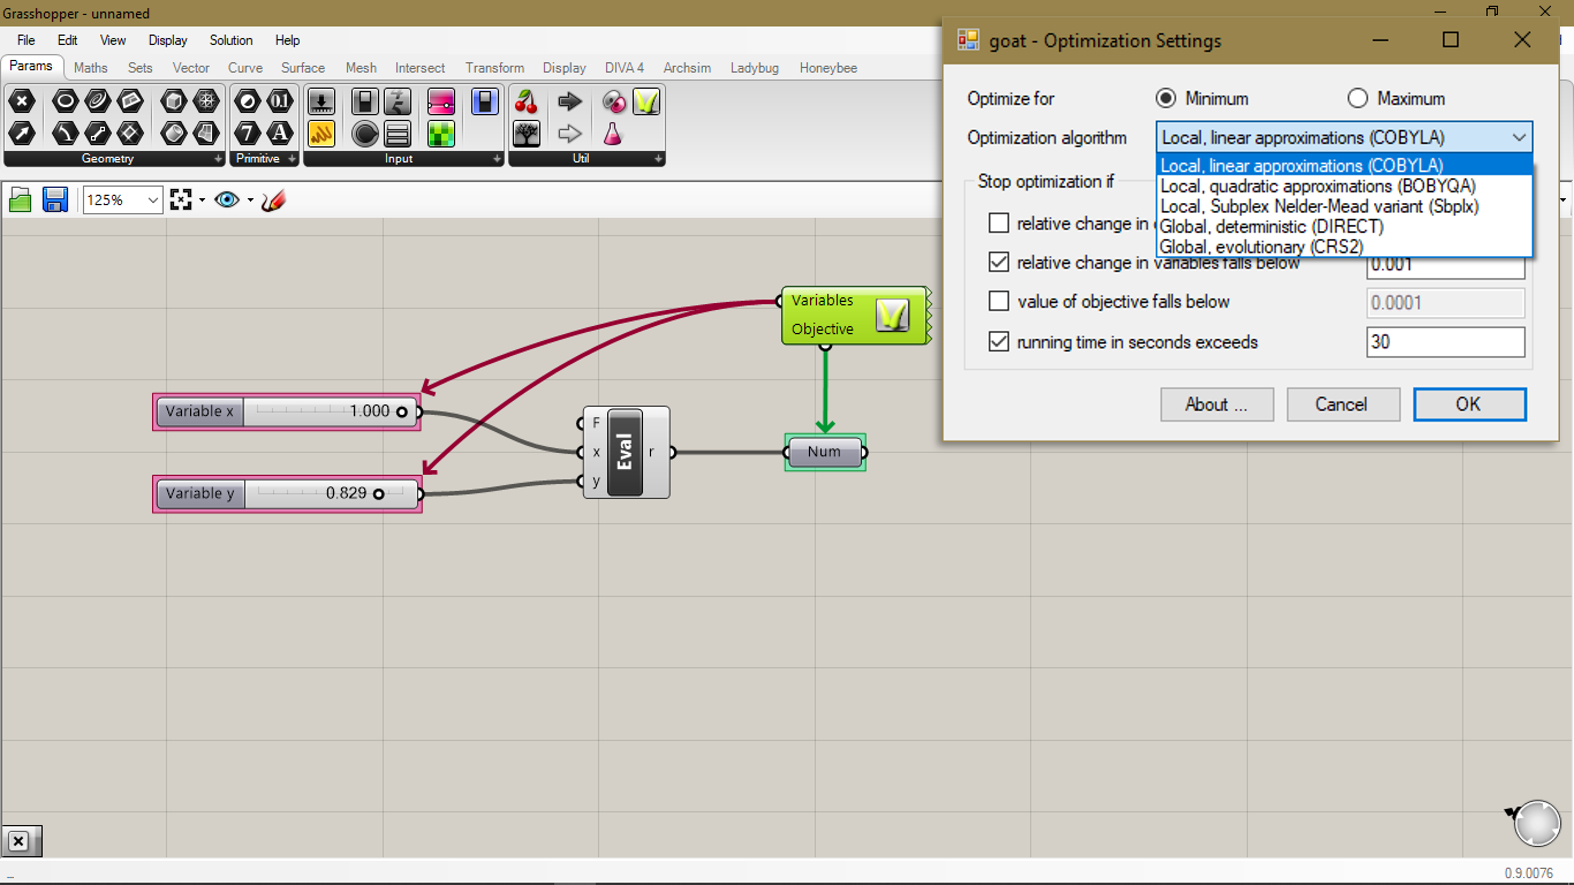
\includegraphics[width=1\textwidth]{Images/Background/Goat/general-view.png}
		\caption[Goat GUI]{Simple view of the Grasshopper's script with the problem definition and the Goat component. On the foreground, the \ac{GUI} exhibits the list of available algorithms within Goat}
		\label{fig:goat}
	\end{figure}
	% End Figure -------------------------------------------------------	
	
	
	% ----------------- [SILVEREYE] ------------------
	\subsection{Silvereye}
	Silvereye \cite{Cichocka2017SILVEREYE} is a generic optimization plug-in, implemented on top of Grasshopper, developed under the same design principles as Galapagos to enable non-experts to solve complex optimization problems. 
	
	Silvereye interfaces a C\# implementation of a global single-objective \ac{PSO} algorithm.
	
	Similarly to the previous tools, Silvereye also requires the definition of the problem in a Grasshopper script, and that the variables and the objective function value are represented by sliders and number components, respectively. Thus, it does not require any additional effort in order to be used.
	
	Likewise Galapagos, the user must double-click Silvereye's component in Grasshopper to visualize its \ac{GUI} (see \Cref{fig:silvereye}). Even though Besides being very simple and intuitive to use, Silvereye also allows less experienced users to start using the tool immediately by providing default values to the extra configuration parameters. As the users gain more experience, they might decide to change some configurations associated with the solver. One other difference to Galapagos is the ability to save the solver's configurations so that it can be used in subsequent runs.
	
	Regarding its visual capabilities, Silvereye is resemblant of Goat, providing no graphical views of the optimization run's state. However, Silvereye does present a list that is updated in real-time with the value of the best fitness value per iteration, which can be exported to a file and then used to create fitness graphs (see \Cref{fig:silvereye2}). Unfortunately, since this file merely contains the fitness values, the user is not able to trace them back to the values of the design parameters which originated them. Moreover, despite the existence of a functionality in the first menu (\Cref{fig:silvereye1}) to create a log file, this file only contains information about the temporal behavior of each evaluation. While this information is useful to monitor and identify irregularities during the optimization run, it does not provide enough information to traceback the error. 
	
	Overall, the lack of visual feedback in the form of graphs hinders the comprehension of and confidence on the results. The ranked list helps filling this gap, as long as there are multiple solutions and the user is able to visualize them in a \ac{CAD} tool.
	
	\begin{figure*}[htbp]
		\centering
		\subfigure[]{%
			\label{fig:silvereye1}%
			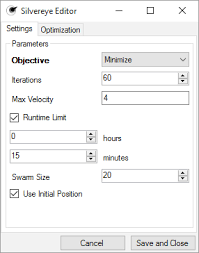
\includegraphics[width=0.40\textwidth]{Images/Background/Silvereye/silvereye.png}}%
		\hfill
		\subfigure[]{%
			\label{fig:silvereye2}%
			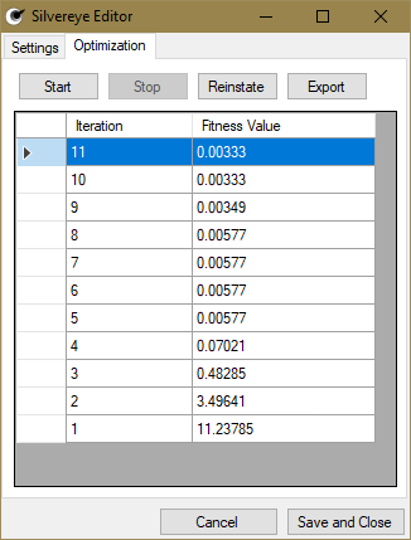
\includegraphics[width=0.40\textwidth]{Images/Background/Silvereye/silvereye2.png}}%
		
		\caption[Silvereye GUI]{Two views of Silvereye's \ac{GUI}: (a) Solvers configuration menu (b) Optimization control and results menu}
		\label{fig:silvereye}
	\end{figure*}
	
	%------------------ OPOSSUM ----------------------
	\subsection{Opossum}
	Opossum (OPtimizatiOn Systems with SUrrogate Models) \cite{Wortmann2017Opossum} is a generic plug-in, developed on top of Grasshopper, that explores Galapagos ideas to confer non-programmers an easy way to tackle a wide variety of problems.
	
	Opossum interfaces that the model-based RBFOpt library \cite{RBFOPT}, exposing two single-objective variants of the global RBF algorithm. 
	
	In terms of usability, Opossum also resembles Galapagos, only requiring the definition of the problem in a Grasshopper script. To use the Opossum's solvers, the user must drag the Opossum's component to the Grasshopper script and connect it with the variables and the objective function components.
	
	Opossum's \ac{GUI} is simple, friendly, intuitive, and well-organized (see \Cref{fig:opossum}). In contrast to other plug-ins, Opossum presents different menus tailored for different levels of expertise. On the one hand, Opossum promotes a ready-to-use format, in order to ensure that less experienced users are able to use Opossum's capabilities. Therefore, Opossum provides two top-level configurations menus for which the values are already filled by default. On the other hand, Opossum provides more experienced users with the ability to create a finer configuration for the optimization solvers and, thus, achieve potentially more efficient optimization processes. 
	
	% Begin Opossum-Options Figure -------------------------------------------------------
	\begin{figure}
		\centering
		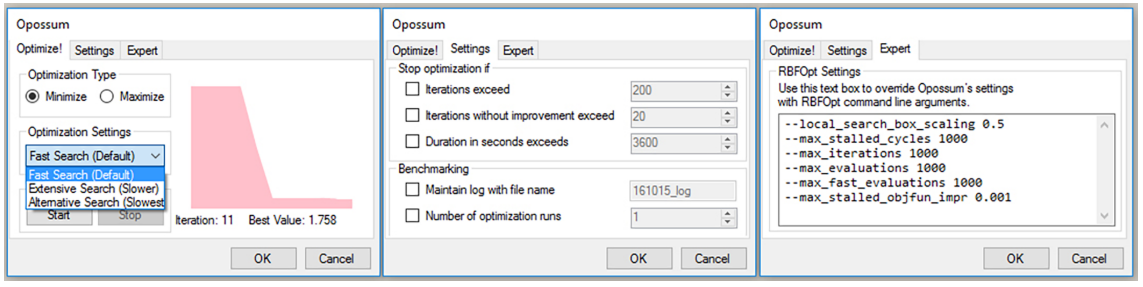
\includegraphics[width=1\textwidth]{Images/Background/Opossum/opossum_1.png}
		\caption[Opossum GUI]{The three views of Opossum's \ac{GUI}. Image retrieved from~\cite{Wortmann2017Opossum}}
		\label{fig:opossum}
	\end{figure}
	% End Figure -------------------------------------------------------
	
	The main deception of this plug-in lies in its visualization features. Although Opossum presents a fitness graph that is very useful for obtaining immediate feedback about the course of optimization, it does not provide an overview of the extent of the design space that is being explored, nor about the distribution of the designs that are being evaluated. Moreover, Opossum supports the creation of a log file that records all the solutions evaluated during the optimization run. Using other post-processing tools, the user can then either produce more insightful visualizations of the data, or re-use this information to create more accurate surrogate models, for example, for sensitivity analysis.
	
	One other disadvantage of this plug-in is the fact that the result of the optimization run is a single solution, instead of multiple ones. As a result, the intelligibility of results and the confidence on the process is greatly hindered, especially, due to its low visual support. 
	
	% ------------- [ Octopus ] -----------------
	\subsection{Octopus}
	
	Octopus \cite{OCTOPUS} is a generic plug-in, developed on top of Grasshopper, that allows non-programmers to address a wide variety of \ac{MOO} problems. 
	
	Octopus exposes two global metaheuristics algorithms, that explore evolutionary principles to search for Pareto-optimal solutions: \ac{SPEA2} and \ac{HypE} algorithms. These algorithms have been reported to yield promising results on numerous \ac{MOO} test problems~\cite{Zitzler2001SPEA2,Zitzler2011HypE}. 
	
	Even though Octopus was originally designed exclusively for optimization purposes, more recently, it focus has grown to include other \ac{ML} utilities, like supervised and clustering mechanisms. In fact, the first difference to the Galapagos-based plug-ins is related to this features' multiplicity, i.e., whereas previous Galapagos-based plug-ins focussed exclusively on optimization, Octopus covers multiple functionalities. This extra functionality is implemented as Grasshopper's components that are made available during Octopus' installation process under a tab that is created within Grasshopper (see \Cref{fig:octopus1}).
	
	The second difference affects the Grasshopper script. Like Galapagos, Octopus does require the definition of a Grasshopper script defining the variables and the objective functions. However, since Octopus focusses on \ac{MOO}, the user has to ensure that all the results of the objective functions are aggregated in single number component and then connected to the Octopus component. Additionally, because Octopus only performs minimizations, the problem definition must be modified to guarantee that all objectives are being minimized. One other important difference is that Octopus is able to tackle constrained problems. In this case, the hard constraints must be represented by a boolean component, and then connected to the Octopus component.
	
	After creating the Grasshopper script, Octopus \ac{GUI} can be accessed by double-clicking the Octopus component (see \Cref{fig:octopus2}). Despite its simplicity and friendliness, the \ac{GUI} is poorly organized and overloaded with information, hence making it difficult for a non-experienced user to locate any functionality in the interface. Although Octopus is distributed in a ready-to-use format, this plug-in exposes mechanisms to fine-tune a few parameters of the solvers. Even more surprising is the ability to change some of these parameters (e.g., elitism, mutation probability, crossover rate, mutation type) during runtime, thus increasing the user interactivity, and allowing the user to influence the optimization process.
	
	Octopus provides good support in terms of graphical feedback, providing three distinct views of the optimization problem (see views 1, 8, and 10 in \Cref{fig:octopus2}), namely:
	\begin{itemize}
		\item Solutions' Objective Space graph, which illustrates the distribution in the objective space of the solutions obtained during the optimization run. This graph also exhibits the approximated Pareto front that is currently known by the algorithm;
		\item Horizontal parallel coordinates graph, which serve the same purpose of the vertical parallel coordinates graph and that provide a view over the different design solutions that have been tested;
		\item Objective convergence graphs (one for each objective dimension), showing the upper- and lower-bounds of the Pareto front (dark gray) and the elite (light gray) of the number of history generations.
	\end{itemize} 
	
	Even though Octopus is capable of solving problems with up to five objective dimensions\footnote{Octopus uses the three spatial dimensions, color, and size to represent the five objective dimensions.}, the readability of these graphs becomes strongly damaged after the three dimensions. Besides the strong visual mechanisms, Octopus provides mechanisms to interact and instantiate each one of the solutions in the corresponding \ac{CAD} tool, which not only gives confidence to the user about the results, but also allows him to understand them better. Optionally, Octopus makes it possible to disable the real-time visualization of the optimization process with the aim of reducing the associated time penalizations.
	
	One other important feature of Octopus is the ability to create logs with the information about the evaluated solutions discriminated by generation. The only setback is that it does not allow to create a single file simultaneously containing the information about the design parameters and the objectives. 
	
	\begin{figure*}[htbp]
		\centering
		\subfigure[]{%
			\label{fig:octopus1}%
			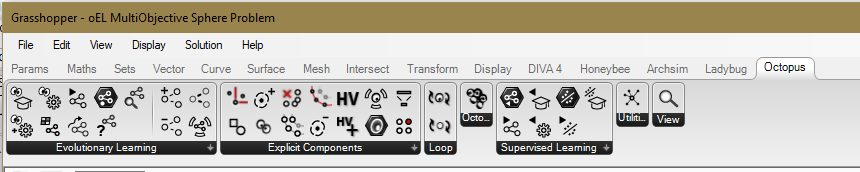
\includegraphics[width=1\textwidth]{Images/Background/Octopus/tab.PNG}}%
		\hfill
		\subfigure[]{%
			\label{fig:octopus2}%
			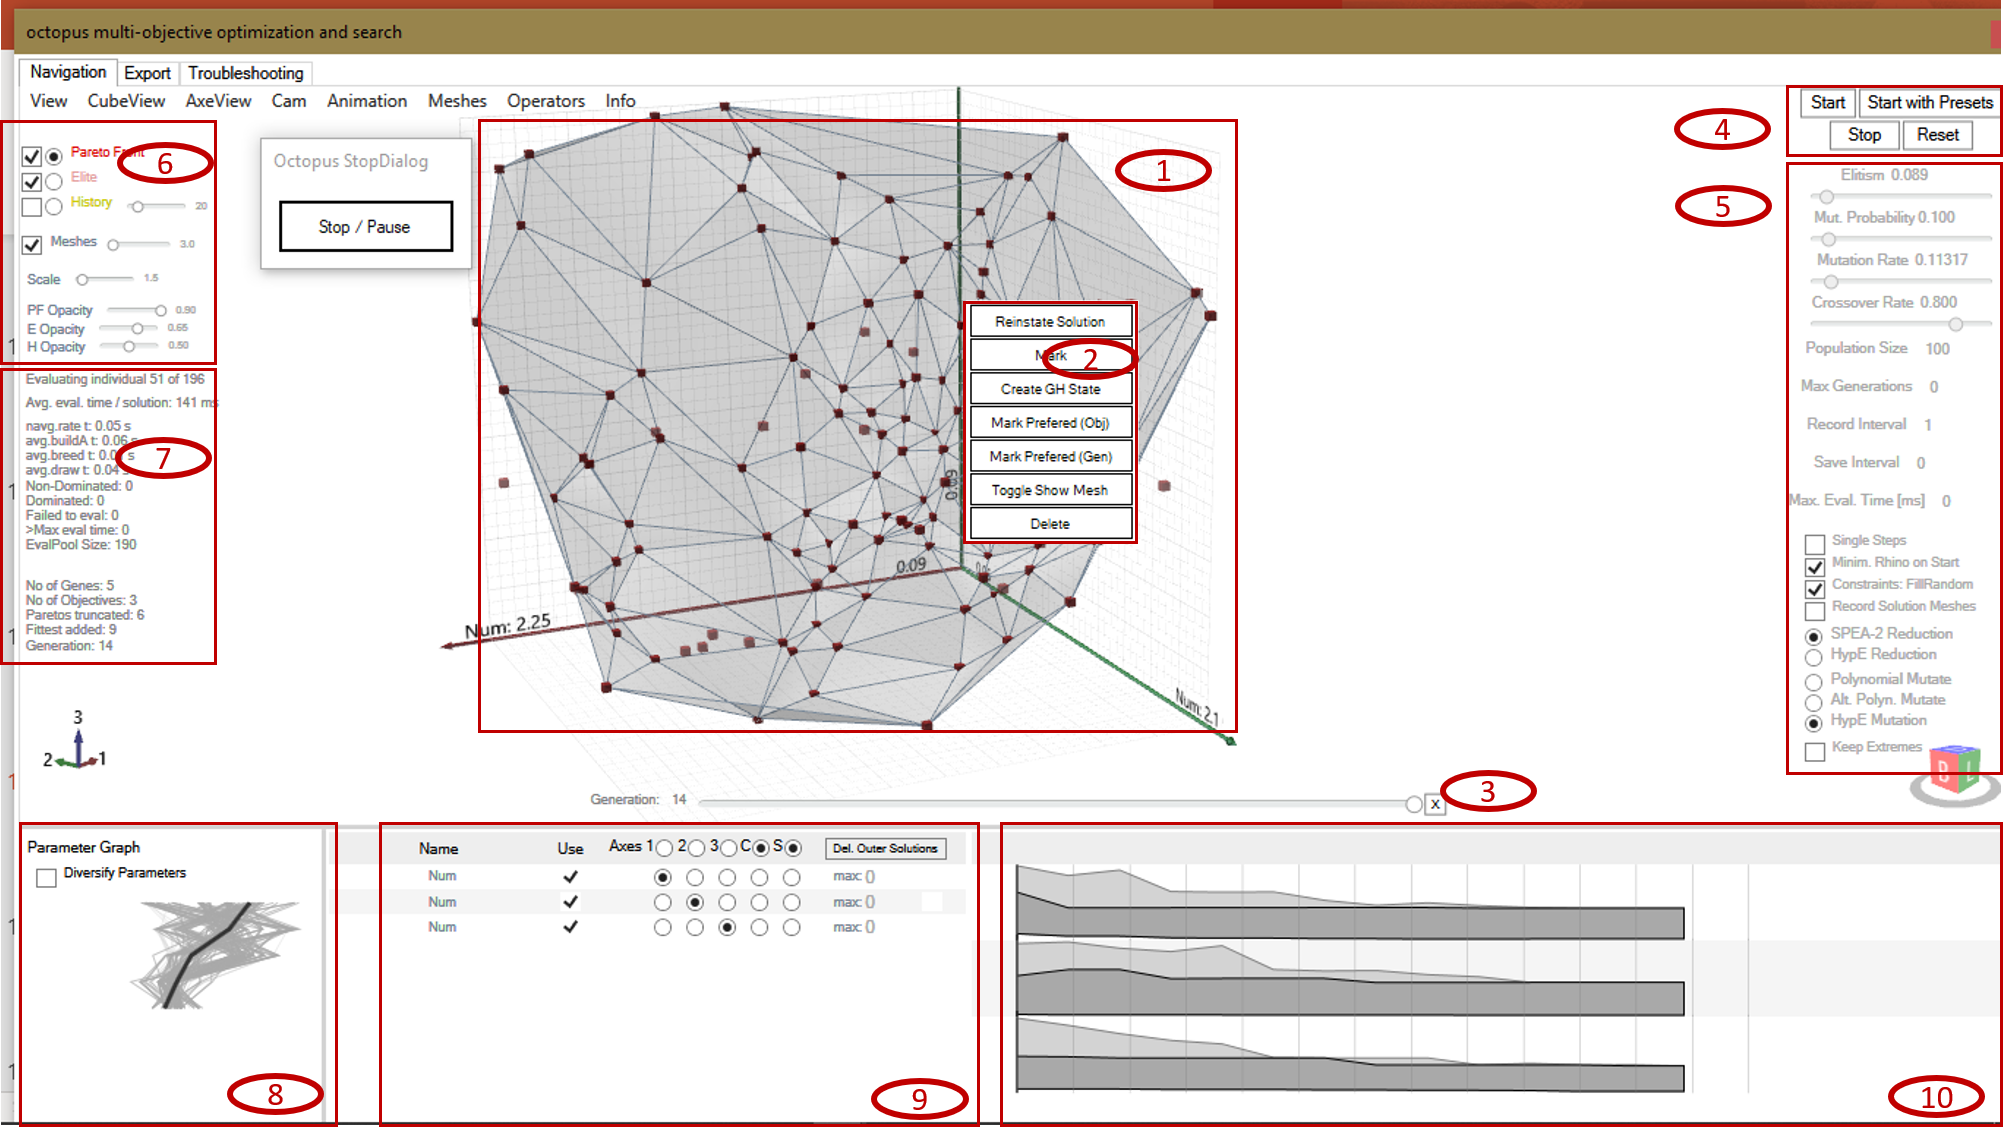
\includegraphics[width=1\textwidth]{Images/Background/Octopus/octopus-menu.png}}%
		\caption[Octopus GUI]{Octopus's \ac{GUI}: (a) Octopus menu in Grasshopper (b) Octopus optimization menu: (1) Solutions' Objective Space, (2) Solution's context menu, (3) Generation's history slider, (4) Process control options, (5) Algorithm Settings, (6) Display Settings, (7) Statistics, (8) Parallel Coordinates Graph, (9) List of Objectives (10) Convergence graphs per Objective}
		\label{fig:octopus}
		
	\end{figure*}
	
	
	% ------- ------- [OPTIMO] -------- ----------
	\subsection{Optimo}
	\label{subsec:Optimo}
	
	Optimo \cite{OPTIMO} is a generic plug-in, implemented on top of Dynamo, that allows non-programmers to address a wide variety of \ac{MOO} problems in the context of a \ac{BIM} tool. 
	
	Optimo interfaces the \ac{MOO} metaheuristics library, jMetal.NET and its current version merely supports the \ac{NSGA-II} algorithm\cite{Deb2002}.
	
	To use the solver, users must create the Dynamo script that encodes the problem definition, but also encode the optimization algorithm. To create the latter, Optimo provides four Dynamo nodes:
	\begin{itemize}
		\item Initial Solution list, which generates the initial set of random design configurations within a provided range and with the specified size of population;
		\item Assign Fitness Function Results, which evaluates and assigns the objective values to each configuration; 
		\item Generation Algorithm, which takes the parent population and generates the children population;
		\item Sorting, which uses the Pareto Front sorting to sort the solutions
	\end{itemize} 
	
	When compared to the previous plug-ins, Optimo demands larger initial investments for the production of the script. As a result, whereas less experienced users might find it more difficult to use, more experienced ones might adjust the algorithm to their needs, which directly results from the finer-grain control of Optimo. Moreover, instead of providing a default template, Optimo foster the constant arrangement of the algorithm's nodes everytime a new optimization process is to be applied, which can quickly become monotonous and tiresome. Moreover, Optimo does not have a explicit \ac{GUI} editor, instead being directly integrated in the Dynamo environment in the form of nodes.
	
	% Visual
	Regarding the visual mechanisms, it does not support feedback mechanisms during the optimization run, only presenting a small side-by-side view of the initial design variation and the optimal designs, thus allowing the user to visualize and compare the results of the optimization process. Finally, we were not able to conclude whether Optimo enabled the creation of log files or not. 
	
	% Comparison
	\subsection{Comparison}
	
	\Cref{table:pluginscompare} shows a comparison between the optimization plug-ins analysed in this chapter at the light of four aspects: (1) the optimization algorithms; (2) the interaction and visualization mechanisms; (3) the comprehension of results; and (4) the user experience.
	
	Taking into account the first aspect, we can observe that most optimization tools focus on single-objective and global optimization. Regarding the diversity of the algorithms most plug-ins provide either one or two options with the exception of Goat which provides five different algorithms from different derivative-free classes. Apart from Goat and Opossum, all other plug-ins support exclusively metaheuristics algorithms.
	
	When considering the interactivity and visualization mechanisms of the explored tools, all plug-ins but Goat yield multiple solutions and allow the user to interact with it and re-instantiate these solutions directly in the corresponding \ac{CAD} or \ac{BIM} tool. Surprisingly, only Galapagos, Opossum, and Octopus present graphical feedback mechanisms. Particularly, Galapagos and Octopus provide not only mechanisms about the state of the optimization (e.g., parameters values being explored, current fitness values), but also provide an overall ranking of the best solutions. On the other hand, none of the plug-ins except for Octopus enable the user to influence and interact with the optimization process during its execution. Even the interactions supported by Octopus are very limited consisting of the modification in runtime of the values of the elitism, mutation, and crossover operators. Regarding the traceability feature (e.g. creation of logs, solutions' lists), it is poorly supported. While Goat has no traceability, both Galapagos and Silvereye provide a ``semi-traceable'' list with the fitness values of the best attained solutions. At last, both Opossum and Octopus support, in a way, the creation of logs describing the state of the whole optimization process, i.e., information about the evaluated design variations with their parameters and corresponding objectives values.
	
	Regarding the third aspect, there are no mechanism explicitly designed to enhance the comprehension of the optimization results in any of the analysed tools. However, the existence of visualization mechanisms like Galapagos and Octopus, do enable a better understanding of the the results. This understanding can be further improved by enabling the direct materialization of such solutions in the corresponding 3D model, so that the user may draw conclusions by comparing different solutions. Despite the absence of visual mechanisms in Octopus, Octopus exhibits the best solutions next to the initial solution, thus allowing the user to compare them and better understand them.
	
	Finally, regarding the user experience, all plug-ins are straightforward to use, except for Octopus and Optimo. Both plug-ins require the user to elaborate the program in order to be run, but they differ, however the former requires a single component to be added, whereas the latter requires the definition of the solver using the provided nodes.
	
	\todo{Tratar disto. Resize box está a escalar a fonte também}
	\begin{table}[]
		\centering
		\resizebox{\textwidth}{!}{%
			\begin{tabular}{cl|cccccc|}
				\cline{3-8}
				\multicolumn{1}{l}{} &  & \multicolumn{1}{c|}{Galapagos} & \multicolumn{1}{c|}{Goat} & \multicolumn{1}{c|}{Silvereye} & \multicolumn{1}{c|}{Opossum} & \multicolumn{1}{c|}{Octopus} & Optimo \\ \hline
				\multicolumn{1}{|c|}{\multirow{4}{*}{Optimization Algorithms}} & Objectives & S & S & S & S & M & M \\
				\multicolumn{1}{|c|}{} & Search & G & GL & G & G & G & G \\
				\multicolumn{1}{|c|}{} & Classes & Meta & ALL & Meta & Model & Meta & Meta \\
				\multicolumn{1}{|c|}{} & Algorithms & 2 & 5 & 1 & 2 & 2 & 1 \\ \hline
				\multicolumn{1}{|c|}{\multirow{4}{*}{Interactivity and Visualization}} & Results & M & S & M & S & M & M \\
				\multicolumn{1}{|c|}{} & Graphical Feedback & +++ & - & - & + & +++ & - \\
				\multicolumn{1}{|c|}{} & Real-time Interactivity & - & - & - & - & + & - \\
				\multicolumn{1}{|c|}{} & Traceability (e.g., logs) & + & - & + & ++ & ++ & ? \\ \hline
				\multicolumn{1}{|c}{Intelligibility of Results} &  & + & - & - & - & + & + \\ \hline
				\multicolumn{1}{|c|}{\multirow{3}{*}{GUI Experience}} & Ease of Use & +++ & +++ & +++ & +++ & ++ & - \\ \cline{2-2}
				\multicolumn{1}{|c|}{} & Intuitive/Organized & ++ & +++ & +++ & +++ & + & + \\ \cline{2-2}
				\multicolumn{1}{|c|}{} & Flexible (e.g., fine-tune) & + & - & + & +++ & ++ & ++ \\ \hline
			\end{tabular}%
		}
		\caption[Comparison between the analysed optimization plug-ins]{A comparison between the analysed optimization plug-ins. S - single, M - multi, G - Global, L - Local.}
		\label{table:pluginscompare}
	\end{table}
	% Falar de cada 
	
	\todo{FIX THIS}
	
	
	One of the key differences between Goat and Galapagos is the number and diversity of the algorithms available. Whilst Galapagos supports two global metaheuristics algorithms, Goat supports five distinct algorithms: one metaheuristic, two direct-search, and two model-based algorithms, called CRS2, DIRECT, SUBPLEX, COBYLA, and BOBYQA, respectively. Due to space constraints, a full description of these algorithms will not be provided, instead we refer the interested reader to the relevant literature.  
	
	One of the main advantages of Goat is the algorithms' diversity. By providing algorithms with different characteristics and strategies, architects can test the suitability of each algorithm to their problem and, thus, select the most effective. The right choice may result in large optimization gains, especially when complex and time-consuming simulations are necessary~\cite{Wortmann2016BBO}. For this reason, and due to the uniqueness of each \ac{BPO}, several authors suggest that the selection of the optimization algorithm should be based on the results of several tests with different algorithms for a fixed number of evaluations or a fixed amount of time~\cite{Hamdy2016,Wortmann2016BBO}. Moreover, the distinction between global and optimal algorithms is also critical when striving for accurate and precise optimal solutions. Most global optimization algorithms invest most of their effort searching for the truly optimal solution across large regions of the search space and rarely focusing on promising regions. Consequently, they might return a not so precise global optimum. To overcome this lack of precision and accuracy, one should apply a local optimization algorithm and provide the globally imprecise optimum as input.
	
	
	%Octopus enables the simultaneous search for more than one objective, producing a set of possible optimal solutions that ideally represent the real trade-offs between each objective. In order to search for the Pareto-optimal solutions, Octopus provides two main evolutionary algorithms: \ac{SPEA2} and \ac{HypE}. On the one hand, due to their population-based nature, evolutionary algorithms are able to approximate the Pareto Front in a single run~\cite{Zhou2011}. On the other hand, these algorithms have been reported to yield promising results on numerous test problems~\cite{Zitzler2001SPEA2,Zitzler2011HypE}.
	
	
	
	
	
	
	

% #############################################################################
\section{Problems to Address}
\label{sec:problemsaddress}

\todo{Reler}	
Despite the existence of both optimization  (e.g., DEAP, MOEAFramework, NLopt, RBFOpt), and visualization (e.g. Matplotlib, Plotly, Seaborn) libraries, architects often lack the programming skills necessary to integrate them into an optimization process. 

% Scalablity, portability, code legibility
Several optimization tools integrated in the architectural design workflow have been proposed throughout the years (see \cref{sec:plugins}). In general, these tools are easy to learn and use, which also results from the fact that they make use of visual programming languages. However, the visual programming paradigm often leads to scalability and program's legibility issues, hence impacting the way users interact with these optimization tools. 

On the other hand, the textual paradigm does not face from these scalability issues. Currently existing textual \ac{AD} tools (e.g., Khepri) do not support optimization, but already provide the primitive mechanisms to create automated optimization processes. Moreover, these tools usually offer portability of their programs, thus allowing architects to visualize and analyze their models in different 3D modeling and analysis tools, without the need to change the program.

% Single-Objective
In contrast to the multi-objective view of most \ac{BPO} problems, where architects aim to optimize multiple aspects simultaneously, most of the currently available optimization tools focus on \ac{SOO}. The usage of these tools to address \ac{MOO} often requires the simplification of the corresponding \ac{MOO} problem either by relaxing the objectives or by assigning preferences to each objective as discussed in \cref{ssec:preferencesarticulation}.

% Global optimization
Most tools exclusively support global algorithms. While global optimization algorithms are good for obtaining close to optimal solutions, these often fail to provide more exact solutions. Particularly, not only are local optimization algorithms able to find more exact solutions but they also do so faster, especially if provided with useful information, such as the starting point.

% Unconstrained Optimization
% Moreover, the analyzed plug-ins do not provide explicit support for hard constraints on the variables, other than the lower and upper bounds on the values of variables. While that suffices for some cases, it is not enough for many other cases in building design, where variables must relate to other according some specific relation (e.g., size of a window must be smaller than the size of the enclosing wall). 

% Metaheuristic Optimization
Also, in terms of the optimization algorithms, most tools adopt metaheuristics algorithms. While these algorithms are flexible and applicable to nearly almost domain, they lack convergence guarantees, often requiring several hundreds or thousands of evaluations to reach good results. Especially for simulation-based problems with time-consuming evaluations, these numbers become a large obstacle. In the \ac{MOO} context, the situation becomes even more complicated, as the number of evaluations is multiplied by at least the problem's number of objectives. This problem can be partially reduced by using model-based algorithms, where a secondary and faster model is used for evaluation.

% Visualization
Regarding the visualization, most plug-ins do not provide enough visual information about the optimization state and the results themselves. Inclusively, most of them generate poorly formatted files with insufficient information, thus impeding to trace back the process and even hindering the comprehension of the results (e.g., associate the design parameters' configurations with the corresponding performance values). Even if users use external tools to produce visualization mechanisms based on the information exported from the optimization plug-ins, these are often only available in the end of the optimization run. As a result, if the computer or system crashes during the optimization run (e.g., energy failure), no log files will be produced and all the information collected will be lost. 

At last, most tools do not offer the possibility for interacting with them, nor do they provide means to pause and resume optimization runs. This is an inconvenience because it impedes users to add the knowledge they have learned, i.e., during the optimization run users would ideally extract information from good visualization mechanisms, that they could add to the process to make it more efficient.

Taking all the \textit{pros} and \textit{cons} of the analyzed tools into consideration, we identify the predominance of metaheuristics algorithms as one of the main drawbacks of currently existing architectural optimization tools, especially when considering \ac{MOO}. Due to the limitations associated with this class of algorithms and time complexity of typical \ac{BPO} processes, the wrong use of these algorithms might lead to dead slow optimization processes, often discouraging its practice. Additionally, there seems to be a generalized lack of standard approach to optimization approaches. As a result, architects tend to adopt the same algorithm for every design, which in this case is the Galapagos' \ac{GA}.  Moreover, given the difficulties and limitations of \ac{MOO}, most \ac{BPO} practicioners opt for \ac{SOO) tools. 
	
This dissertation addresses the time complexity of problems involving costly evaluation functions, especially, when considering \ac{MOO}. In the next chapter, we present our solution.
%In the next chapter, we describe the architecture of our solution and explain how each component achieves the features highlighted in this section.
